\documentclass[11pt, oneside]{article}   	
\usepackage{geometry}                		
\geometry{letterpaper,margin=1in}
\usepackage{authblk}
\usepackage{graphicx}						
\usepackage{bm}
\usepackage{amssymb}
\usepackage{float}
\usepackage{array}
\usepackage{xcolor, colortbl}
\usepackage{rotating}
\usepackage{multirow}
\usepackage{amsthm}
\usepackage{amsmath}
\usepackage{amssymb}
\usepackage{natbib}
\usepackage{minted}
\usepackage[section]{placeins}
\usepackage{colonequals}
\usepackage{ctable}

%\usepackage{hyperref}
%\hypersetup{
%    colorlinks=true,
%    linkcolor=blue,
%    filecolor=magenta,      
%   urlcolor=cyan,
%}
%\urlstyle{same}

\usepackage[font={small}]{caption, subcaption}

\usepackage[titletoc,title]{appendix}
\PassOptionsToPackage{hyphens}{url}
\usepackage[colorlinks=true,allcolors=black,breaklinks=true]{hyperref}
%\usepackage{breakurl}
%\usemintedstyle{tango}
\newcolumntype{C}[1]{>{\centering\arraybackslash}m{#1}}
\providecommand{\keywords}[1]{\textit{Keywords:} #1}

\definecolor{light-gray}{gray}{0.9}

\theoremstyle{definition}
\newtheorem{definition}{Definition}[section]

\newcommand{\knots}{\mathcal{Q}}
\newcommand{\pp}[1]{\mathcal{\tau}^{#1}}
\newcommand{\rem}[1]{\mathcal{\delta}^{#1}}
\newcommand{\kn}[1]{\knots^{#1}}
\newcommand{\jm}{j_1, \dots, j_m}
\newcommand{\jk}{j_1, \dots, j_k}
\newcommand{\jM}{j_1, \dots, j_M}
\newcommand{\reals}{\mathbb{R}}
\newcommand{\domain}{\mathcal{D}}
\newcommand{\bs}{\textbf{s}}
\newcommand{\bx}{\textbf{x}}
\newcommand{\by}{\textbf{y}}
\newcommand{\bb}{\textbf{b}}
\newcommand{\bK}{\textbf{K}}
\newcommand{\bB}{\textbf{B}}
\newcommand{\bI}{\textbf{I}}
\newcommand{\bfmu}{\textbf{\mu}}
\newcommand{\E}[1]{\mathbb{E} \left[ #1 \right]}
\newcommand{\normal}[3]{\mathcal{N}_{#1} \left(#2, #3 \right)}
\newcommand{\supp}[1]{\text{supp}(#1)}
\newcommand{\Var}[1]{\text{Var}\left( #1 \right)}
\newcommand{\MRATree}{\mintinline{python}{MRATree }}
\newcommand{\MRANode}{\mintinline{python}{MRANode }}
\newcommand{\bfun}[2]{\bb^{#1}_{#2}}

\newcommand{\todo}[1]{\textcolor{red}{[#1]}}
\newcommand{\ann}[1]{\textbf{\color{orange} [Ann: #1]}}
\newcommand{\trey}[1]{\textbf{\color{blue} [Trey: #1]}}
\newcommand\ChangeRT[1]{\noalign{\hrule height #1}}

\title{Extreme Ozone Event Change Point Analysis}
\author[1]{Hugh McCreery \thanks{hughmccreery@mines.edu}}
\author[1]{Baylee McKinney \thanks{bmckinney@mines.edu}}
\affil[1]{Colorado School of Mines Department of Applied Mathematics and Statistics}
\date{}						

\begin{document}
\maketitle
\begin{abstract}
The Tropospheric Ozone Assesment Report (TOAR) provides important metrics and observations of tropospheric ozone worldwide. This report uses the data from the TOAR database to analyze the behavior and trends of ozone. Time series and change point analysis is performed on the data to find when exactly changes in mean ozone levels are occurring. Clustering is then performed on the change points and their amount of change in ozone to find spatial and other trends. After clustering two influential areas are chosen to be examined further, the Ohio Valley and Southern California. 

\smallskip
\keywords{Tropospheric Ozone, TOAR, Time Series, Change Point, Clustering}
\end{abstract}

\newpage

\tableofcontents

\newpage

\section{Introduction} % more general info - from Dr. Cooper's paper
Tropospheric and other ozone is a large contributor to both ecological and health problems. The Tropospheric Ozone Assessment Report (TOAR), contains a database with worldwide ozone metrics and observations. Ozone when in the stratosphere absorbs harmful UV radiation, but ozone in the troposphere can have harmful impacts on the human respiratory and cardiovascular systems (\cite{fleming}). Effects of high ozone levels on the ecosystem includes plant toxicity,changes in rates of chemical and biochemical processes, and ecological interactions (\cite{ecological}). Due to these 2 large factors we believe it is important to examine how and when ozone levels are changing. With ozone levels rising in some portions of the world and falling in other portions of the world it is important to review it's behavior in order to decrease  the ecological and health related impacts.


\subsection{Research Goal} 
Our research goal is to use time series to analyze the locations of potential changes in the behavior of ozone. We're interested in these changes as they could potentially be examined to determine the cause of them. For example, we could examine if changes in ozone metrics have any relationship to economic or population metrics. In this paper we will look at using time series and change point analysis to find significant changes in ozone levels and then examine the patterns and causes of these changes. The discoveries from this analysis could aid in the decrease of ozone levels worldwide.

\subsection{Data}
The data we are going to use will come from the TOAR database (\cite{schultz2017apmd}). The variables we have decided to use to classify and explore change points in ozone levels are the number of days above 70 ppb and the average daily maximum 8-hour average ozone mixing ratios (abbreviated dma8). The number of days above 70 ppb will allow for identification of location specific extreme events that occur occasionally, while the daily maximum mixing ratios will allow us to explore the long term exposure and effects of ozone. The database has information dating back to 1971 but the majority of the stations began tracking in 1980.

We also decided to explore the NetCDF data available from the TOAR database and see if it would offer any additional information or insight. The NetCDF data provided only contains information on the average value of daily maximum 8-hour average ozone mixing ratios and not the days above 70 ppb. Therefore, we decided that the NetCDF data would not provide more useful information to our project and we will not be moving forward with analyzing it. 

\section{Statistical Methods}
\subsection{Time Series}
We are planning on considering the ozone data as a time series for our analysis. Any data which consists of observations of the same variable over time can be analyzed as a time series by not assuming each observation is independent. Not making this assumption allows us to examine if there's any change in the ozone levels over time. Currently we're considering the average daily 8-hour mixing ratios at each station with more than 25 years of data.

\subsection{Change Point Detection}
Change point detection is used on time series data in order to observe changes in the mean or variance of the data. In the instance of ozone behavior, we will be focusing on the detection of change in mean of the time series. We will be exploring methods to detect both single and multiple change points in a single series. Information on these methods are outlined below. Both of these methods come from the R package named change point; more information on this package is given by the authors in this paper (\cite{changepoint})

\subsubsection{At Most One Change (AMOC)} % changepoints harder to detect at beginning/end of TS
To detect if a single change exists in the ozone levels we will use the AMOC method from the changepoint package. This method works by testing each point to determine the likelihood that the distribution of the data before that point differs from the distribution after that point (\cite{changepoint}). Having tested all of the points, the method will either return the year which is most likely to be a change point if that meets a certain threshold value. For example, we've included plots of two series of our dma8 data. The first series are dma8 measurements taken from NOAA's American Samoa Observatory and don't have any change in mean over the sample. The other series are dma8 measurements taken about 50 miles east of Los Angeles. This is an area which has seen a drop in pollution levels and our change point method estimates this change in mean pollution was most likely to have occured in 1994.
% note that it's yearly data
\begin{figure}[ht]
    \centering
    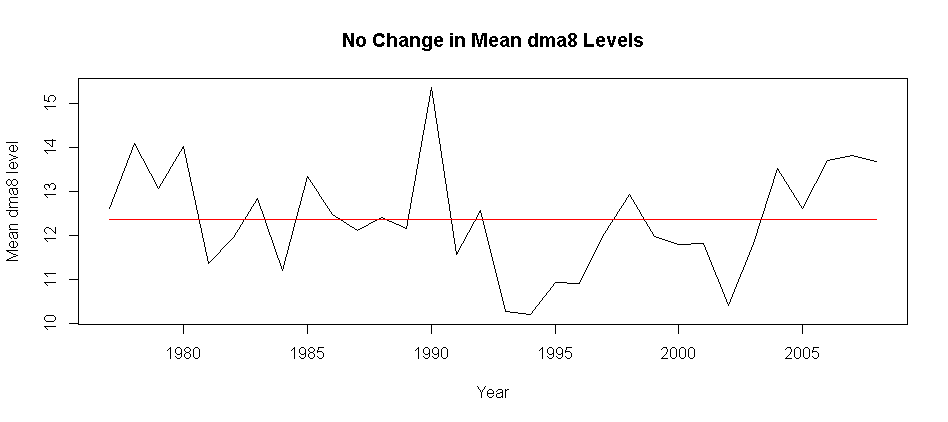
\includegraphics[width=\linewidth]{plots/time_series/SMO514S00.png}
    \caption{Station located in American Samoa; no change in mean dma8 levels}
    \label{ts_samoa}
\end{figure}

\begin{figure}[ht]
    \centering
        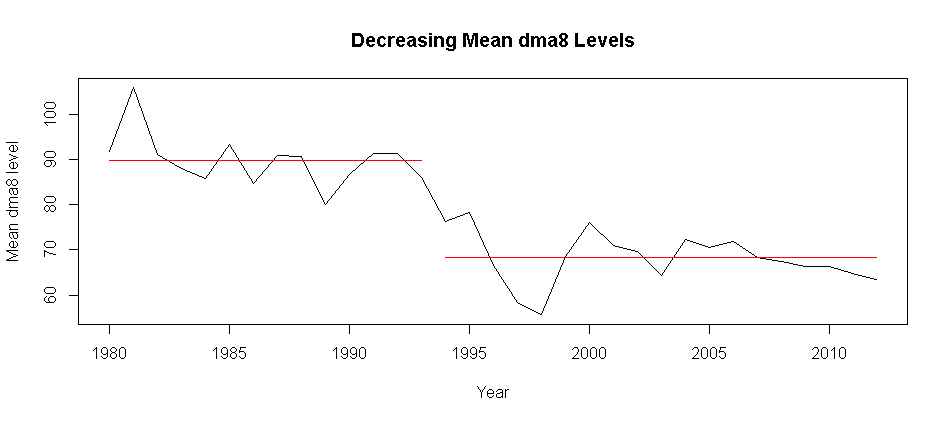
\includegraphics[width=\linewidth]{plots/time_series/06-065-6001.png}
    \caption{Station located outside of LA; decrease in dma8 levels}
    \label{ts_la}
\end{figure}

There are a variety of tests and thresholds that can be used - we're currently testing using the asymptotic penalty and accepting change points if they meet the 95\% confidence levels, but we would like to further examine how the level and test statistic impacts the analysis.

\subsubsection{Pruned Exact Linear Time (PELT)}
The PELT method finds multiple change points in a time series through cost minimization. Detection of change point is more likely with a larger magnitude. Overall PELT is a fast and accurate method for detecting multiple change points in a time series (\cite{pelt}). The main reason for using the PELT method in our analysis is to look at the occurrence and distribution of time series containing multiple change points. 

\section{Findings}
\subsection{AMOC Method}
We first examined the distribution of the change points for the AMOC method both between years and in space. There were two stations for which we estimated that there were no change points and 501 that had at least one point meet the threshold. Below are plots showing how the magnitudes of the changes were distributed across North America and another that shows the frequencies of positive and negative changes globally from 1970 to 2015. We can see that the points with significantly negative changes are clustered in southern California, but on the whole there isn't much of an apparent spatial pattern. 
 
\begin{figure}[H]
    \centering
    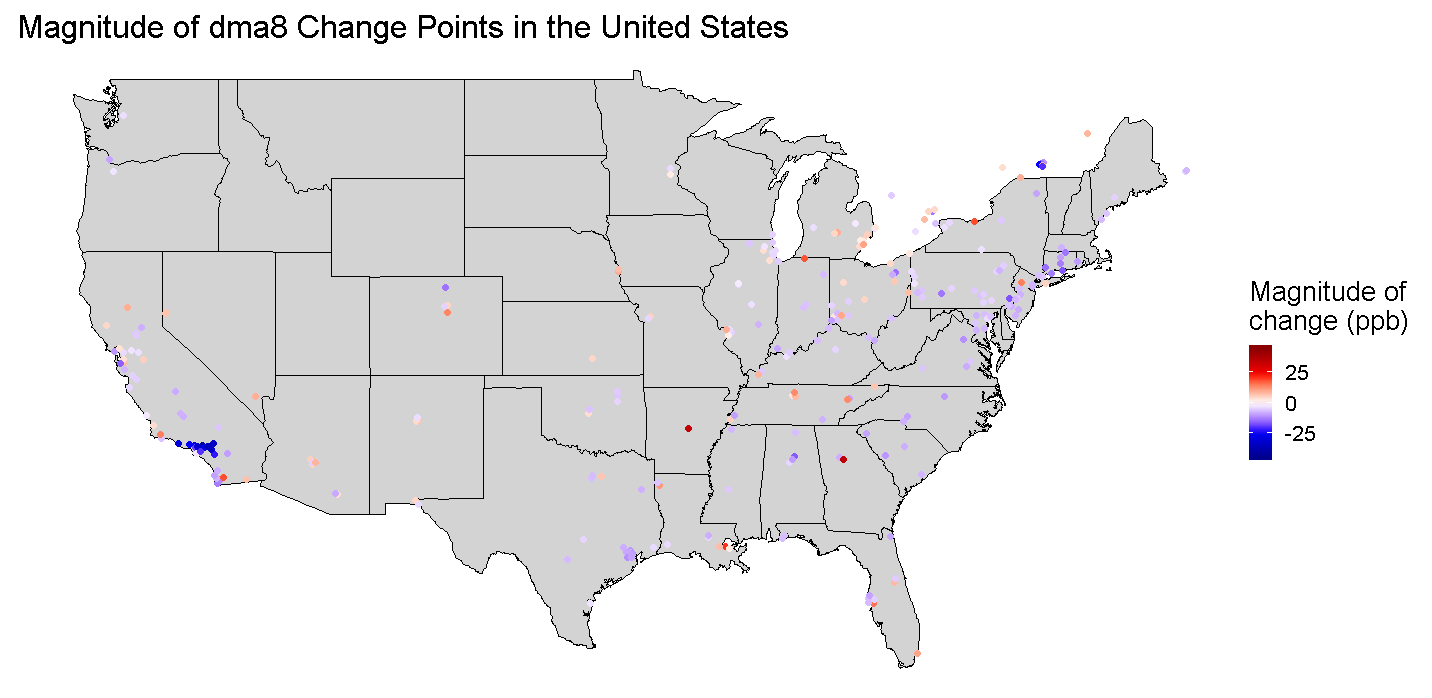
\includegraphics[width=0.75\linewidth]{plots/amoc_na_magnitude_pretty.png}
    \caption{Magnitude of change in daily 8-hour mixing ratio in North America}
    \label{dma8_na}
\end{figure}

We next examined the number of stations that had a change point in each year relative to the number of stations taking measurements at that year. A histogram of the total number of each stations measuring for each year was included for reference. Note that 1975 has the highest percent of stations but this is due to a smaller number of measurements in this year relative to others. We also see a spike in change points in the year 2000. Finally, we see that after 2010 there are relatively few change points as there typically isn't enough data after those years to conclude that a change in mean existed in that year.

\begin{figure}[H] % relative frequencies/line of # stations
    \centering
    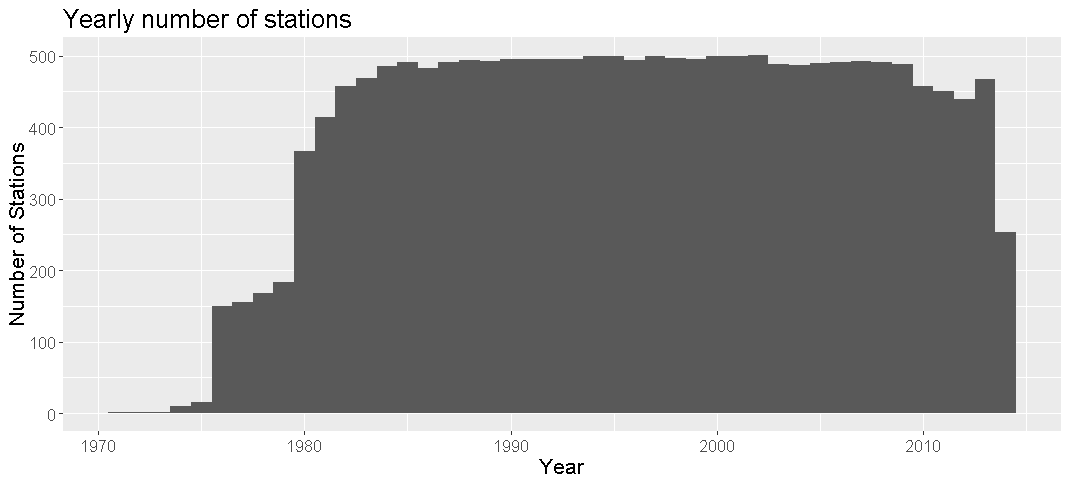
\includegraphics[width=0.7\linewidth]{plots/total_stations.png}
    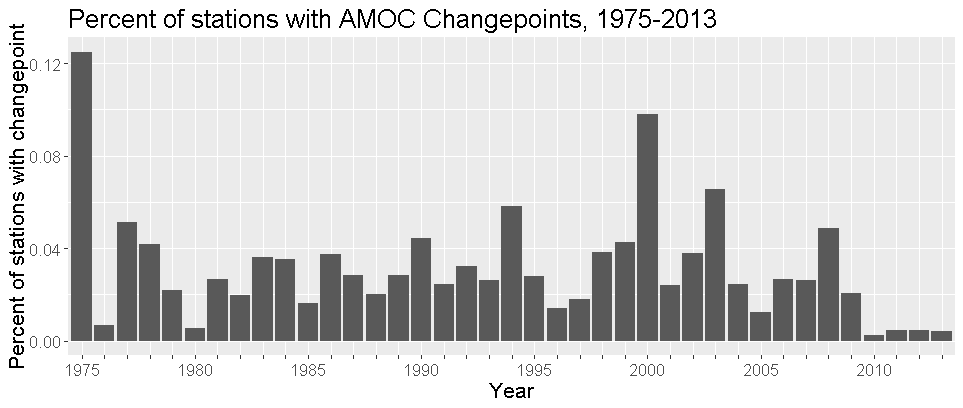
\includegraphics[width=0.7\linewidth]{plots/amoc_hist_relative.png}
    \caption{Histograms of total stations each year and years change points occur in with AMOC Method}
    \label{amoc_hist_rel}
\end{figure}

We also wanted to see if there was any apparent relationship in the direction of each change rather than just if a change existed. Below is a histogram which shows the frequency of positive and negative estimated changes using the AMOC method. We can see that there are a significant number of decreases in the means after the year 2005.

\begin{figure}[H]
    \centering
    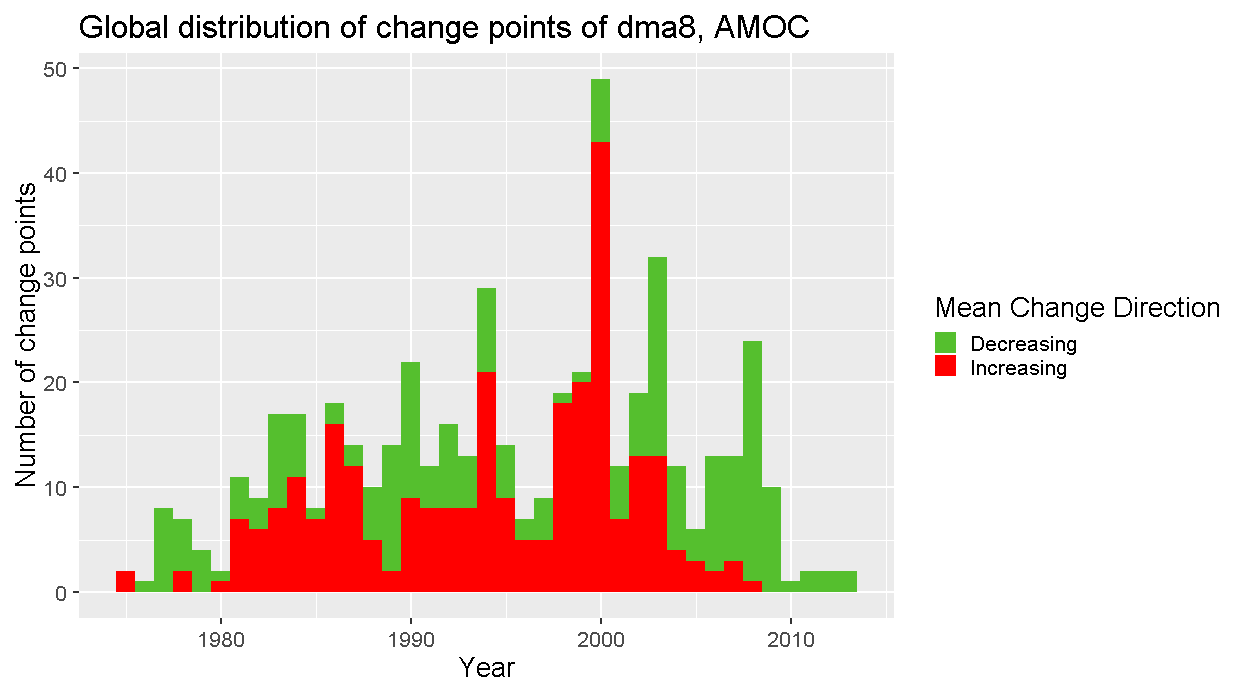
\includegraphics[width=0.8\linewidth]{plots/change_direction_AMOC.png}
    \caption{Histogram of Direction of Change Point in Mean Using AMOC}
    \label{amoc_hist_dir}
\end{figure}

Further exploring the direction of change point, we plotted the change point in mean direction for stations within the US. This is shown in the figure below with red representing a positive change in mean and green representing a negative change in mean. The green color is representing all locations where ozone levels decreased when the AMOC method was used. The number of stations where the change in mean was negative (green points) was 211, while the number of points where change was positive (red points) is 84. This shows that while worldwide the number of positive and negative changes may be more proportionately even, in the US there are a significantly more stations with a negative change in mean than positive.  

\begin{figure}[H]
    \centering
    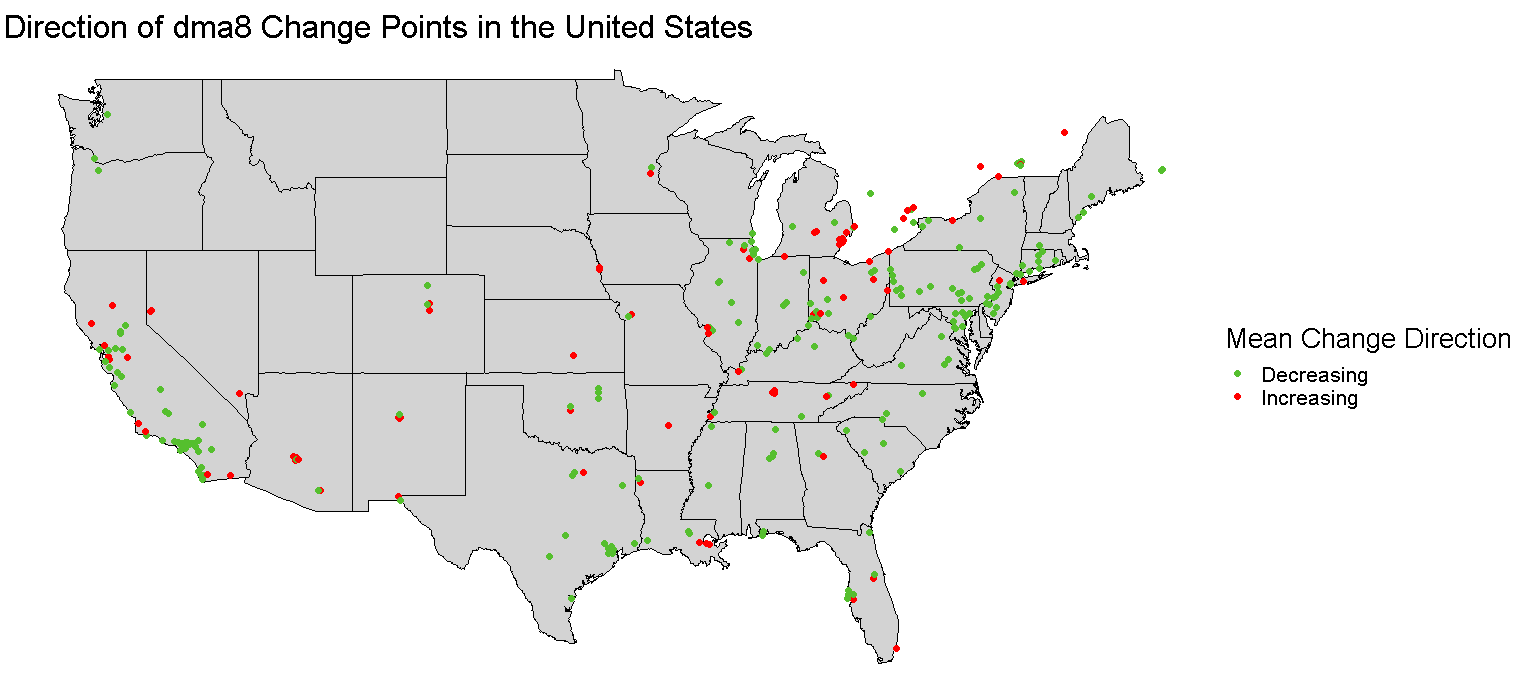
\includegraphics[width=0.7\linewidth]{plots/direction_change_point_US_pretty.png}
    \caption{Direction of Change Point in Mean Shown on US Map}
    \label{amoc_geo_dir}
\end{figure}

\subsection{PELT Method}
In order to analyze the number of change points in a given year using PELT method, we created a histogram. The histogram shown in the figure below allows us to visualize the frequency of change points for each year between 1970 and 2014, with the same total number of station histogram for reference. The frequency of change points appears to have a downward trend after 1990 with a small peak in 2000. This graph is interesting but there may be more information in a histogram that also indicates the direction of the change in mean.
\begin{figure}[ht]
    \centering
    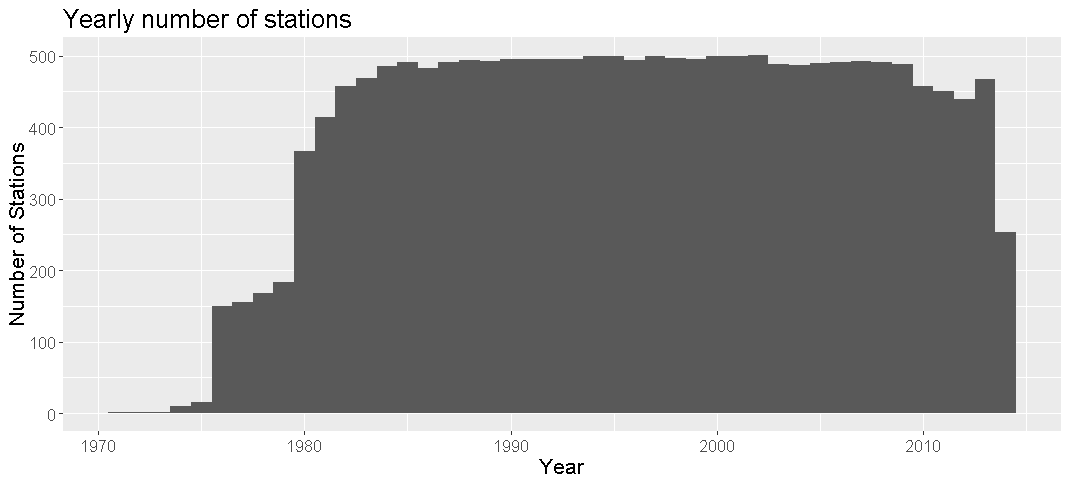
\includegraphics[width=0.7\linewidth]{plots/total_stations.png}
    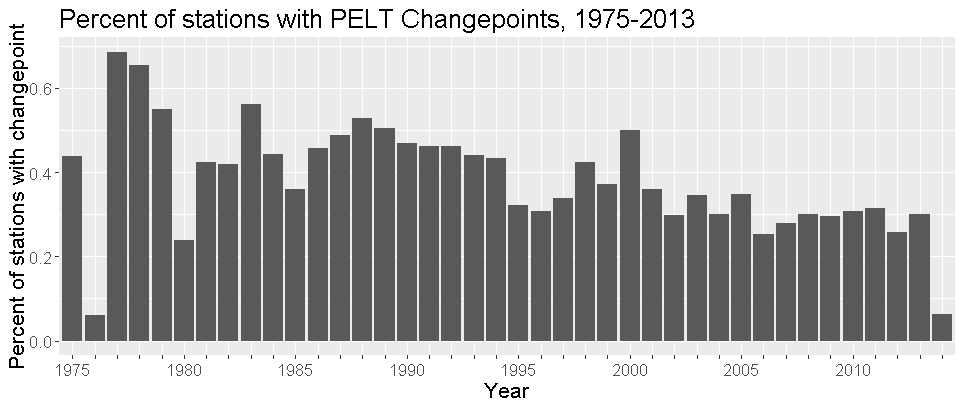
\includegraphics[width=0.7\linewidth]{plots/pelt_hist_relative.png}
    \caption{Histograms of total stations each year and years change points occur in with PELT Method}
    \label{pelt_hist_rel}
\end{figure} \newline
% restate station count
Next, we created a histogram that differentiates change points by the direction of the change in mean. This is shown in the figure below, with the green area representing a negative change in mean and the red area representing a positive change in mean. There were 3,351 change points that had a negative change in mean and 3,227 change points with a positive change in mean. These change points occur over all stations with some stations having multiple change points. There is not a significant difference between the number of stations with a positive or negative change in mean which leads us to believe we need to do deeper analysis than just looking at the direction of the change points when using PELT. Currently our focus is to continue our analysis using the AMOC method for detecting change points, but we hope to expand our research in the future to contain the PELT method. 
\begin{figure}[ht]
    \centering
    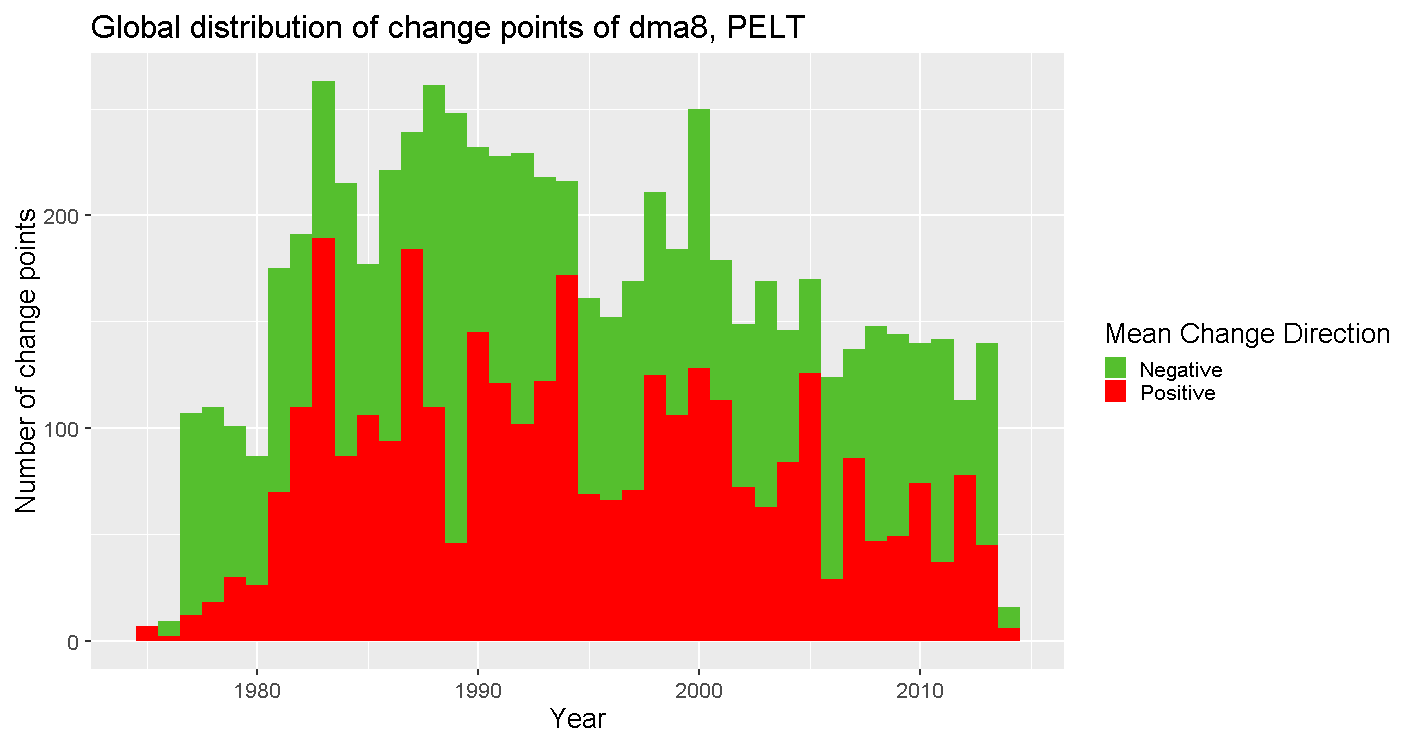
\includegraphics[width=0.8\linewidth]{plots/change_direction_PELT.png}
    \caption{Histogram of Direction of Change Point in Mean Using PELT}
    \label{pelt_hist_dir}
\end{figure}

\section{Clustering}
\subsection{Motivation}
Having found change points for stations using the AMOC method, we next decided to look at clustering these change points to attempt to find any underlying structure. This was done to see if the magnitude and direction of these points generally changed over time, as the result that there were locations with increasing means in the United States (as shown in Figure \ref{amoc_geo_dir}) was surprising. To get an idea of this, the magnitudes of changes in means were plotted (similar to Figure \ref{dma8_na}) but separate it into three different time periods - before 1990, during the 1990s, and after 2000. These plots are shown below. Additionally, we created a scatter plot showing the relationship between the year and magnitude of the changes.

\begin{figure}[H]
    \centering
    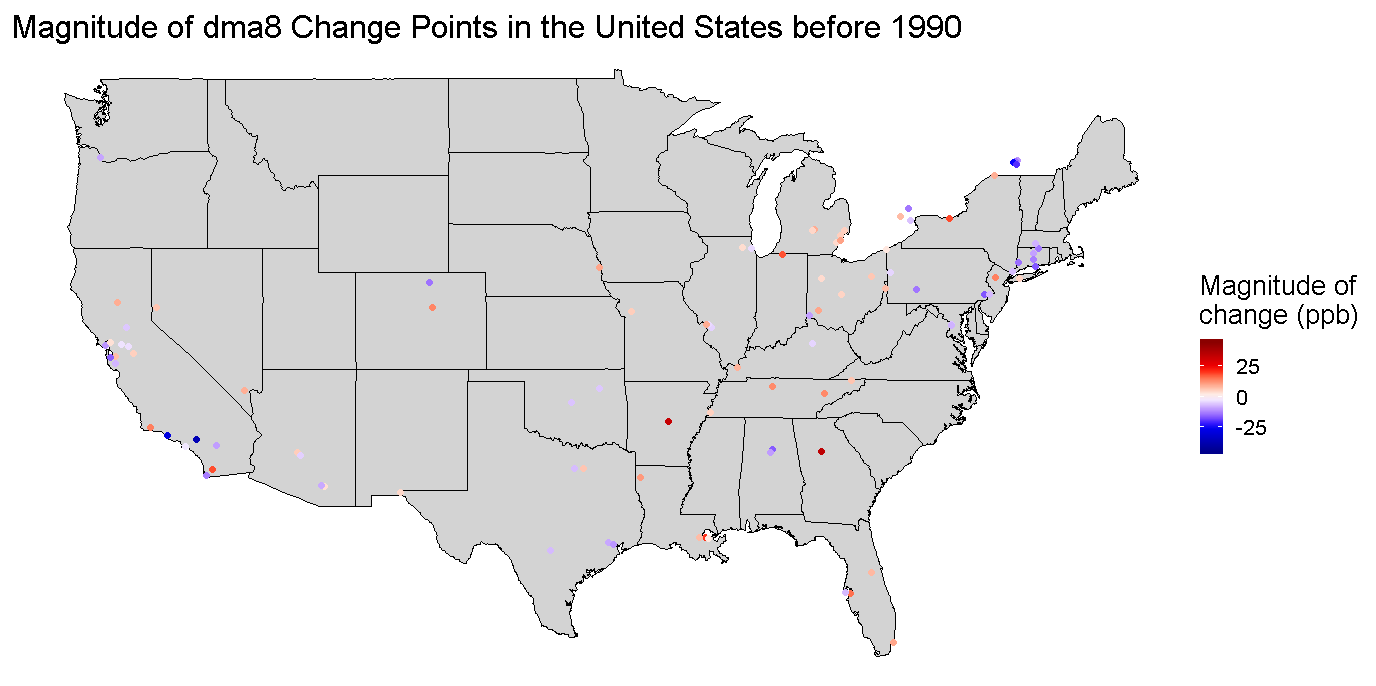
\includegraphics[width=0.8\linewidth]{plots/clustering/changes_before_1990.png}
    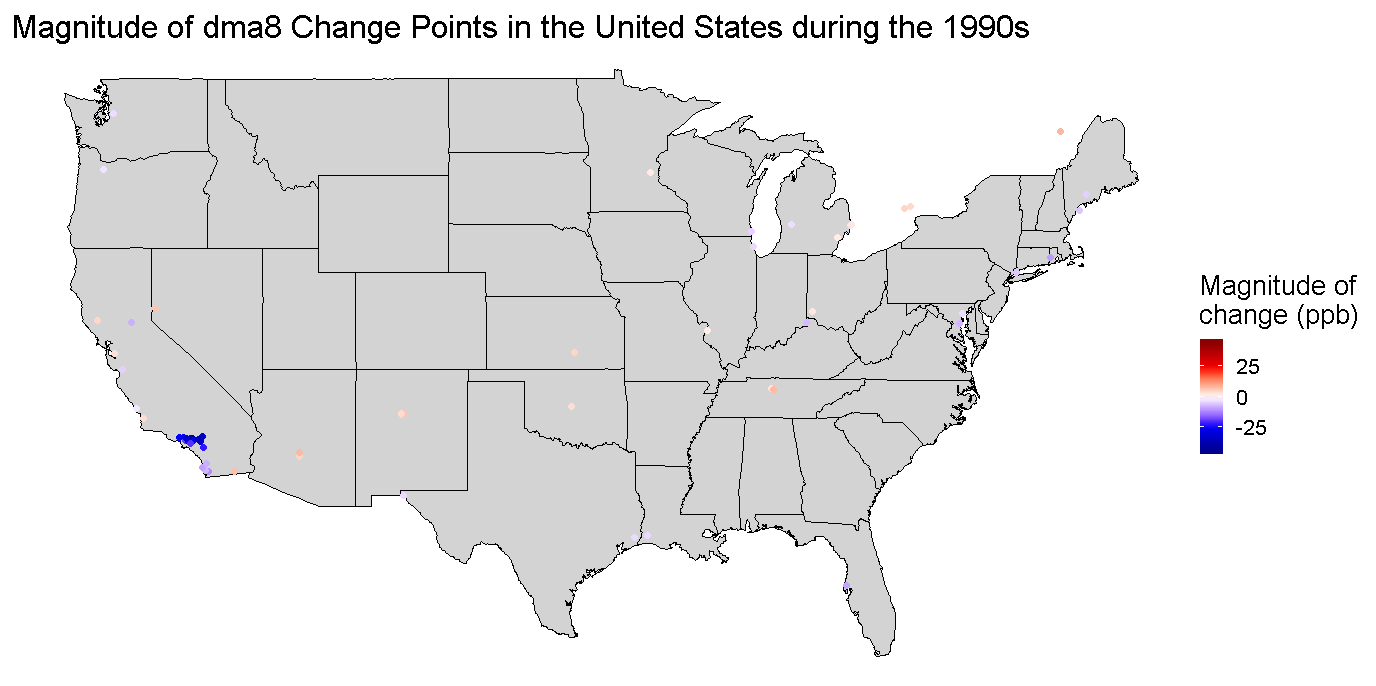
\includegraphics[width=0.8\linewidth]{plots/clustering/changes_during_1990s.png}
    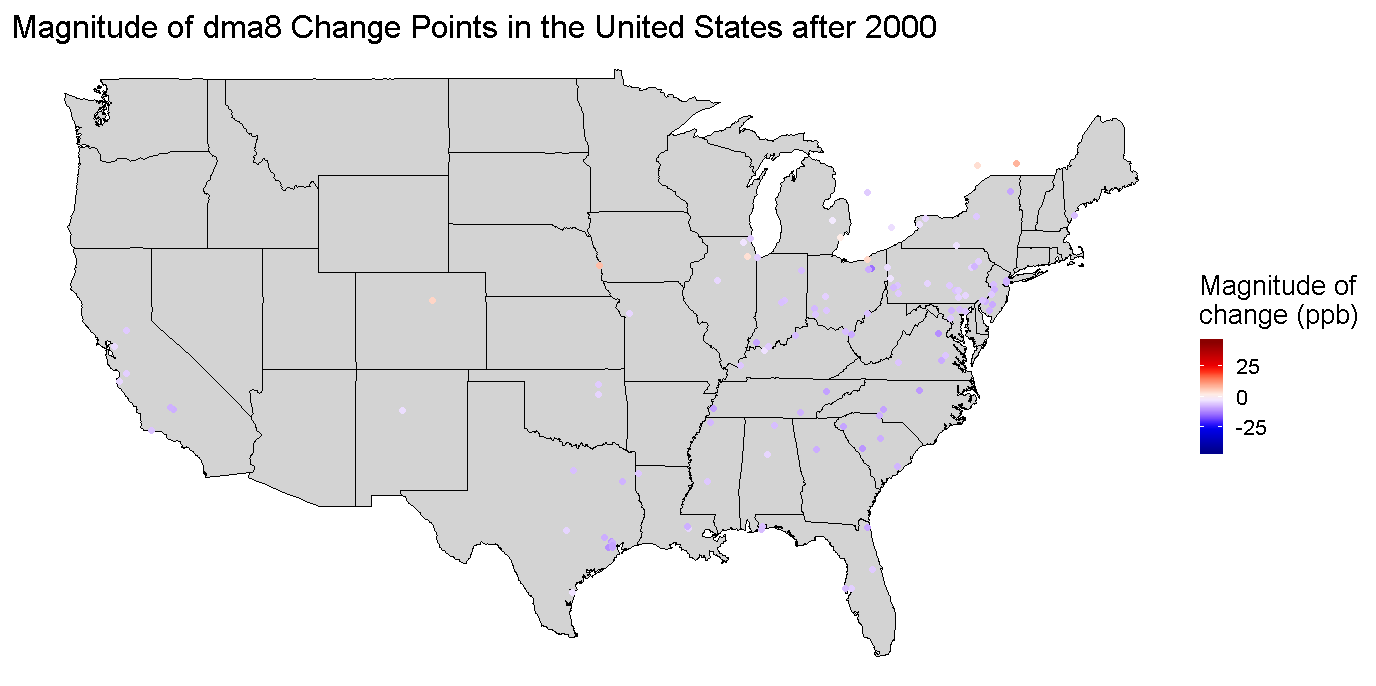
\includegraphics[width=0.8\linewidth]{plots/clustering/changes_after_2000.png}
    \caption{Magnitude of change in daily 8-hour mixing ratio before, during, and after the 1990s}
    \label{na_dma8_changes}
\end{figure}

%\begin{figure}[ht]
%    \centering
%    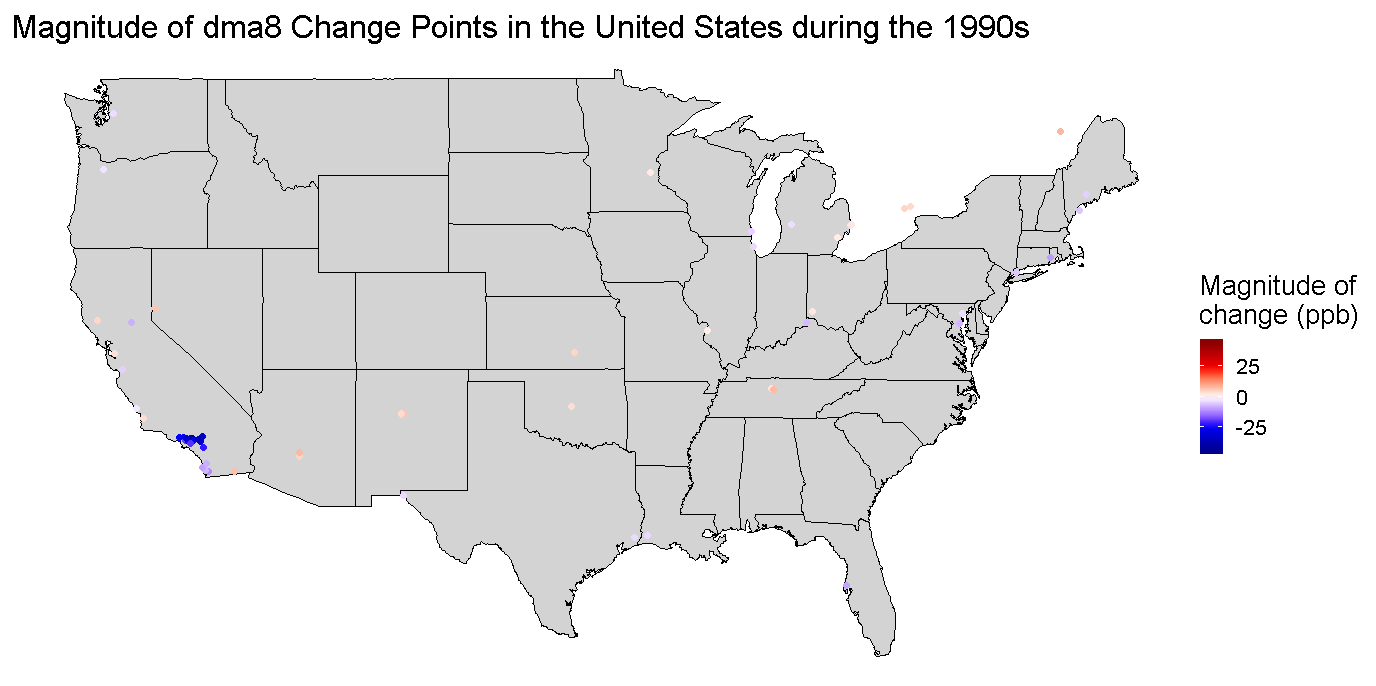
\includegraphics[width=0.7\linewidth]{plots/clustering/changes_during_1990s.png}
%    \caption{Magnitude of change in daily 8-hour mixing ratio, 1990-1999}
%    \label{during_90s_changes}
%\end{figure}

%\begin{figure}[ht]
%    \centering
%    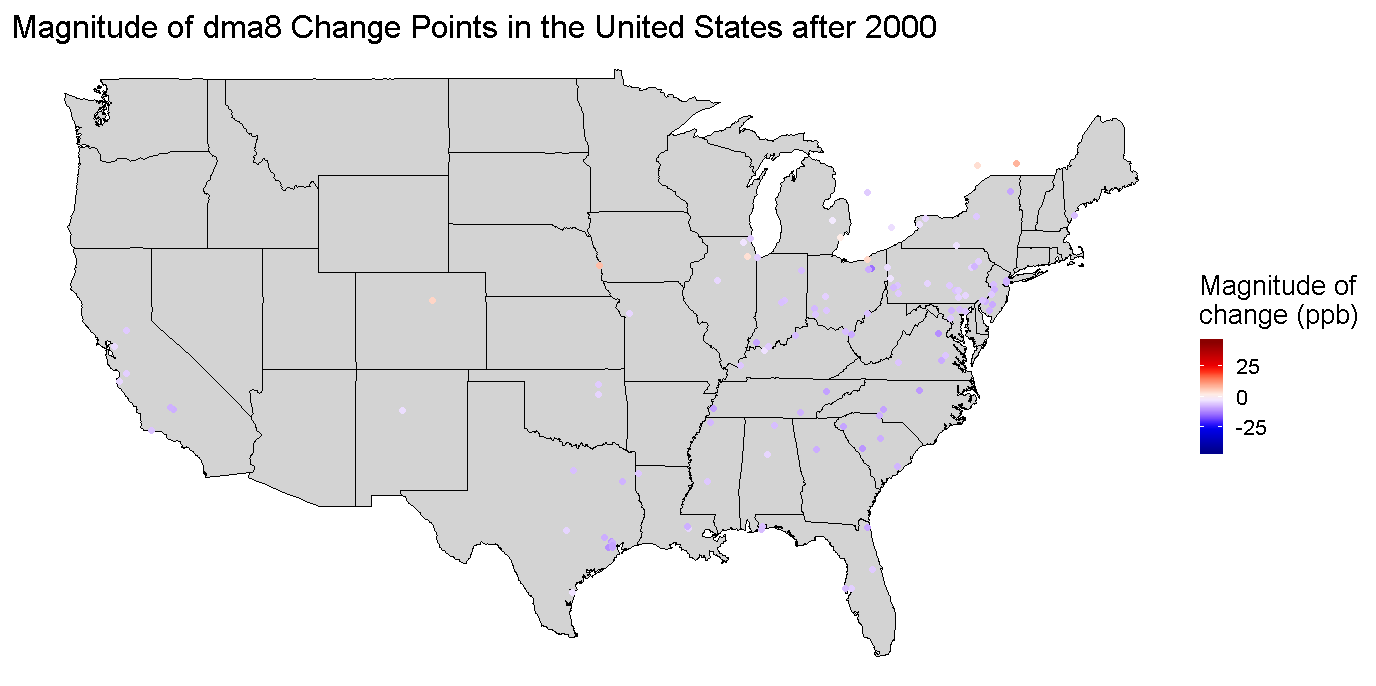
\includegraphics[width=0.7\linewidth]{plots/clustering/changes_after_2000.png}
%    \caption{Magnitude of change in daily 8-hour mixing ratio, after 2000}
%    \label{after_2000_changes}
%\end{figure}

\begin{figure}[H]
    \centering
    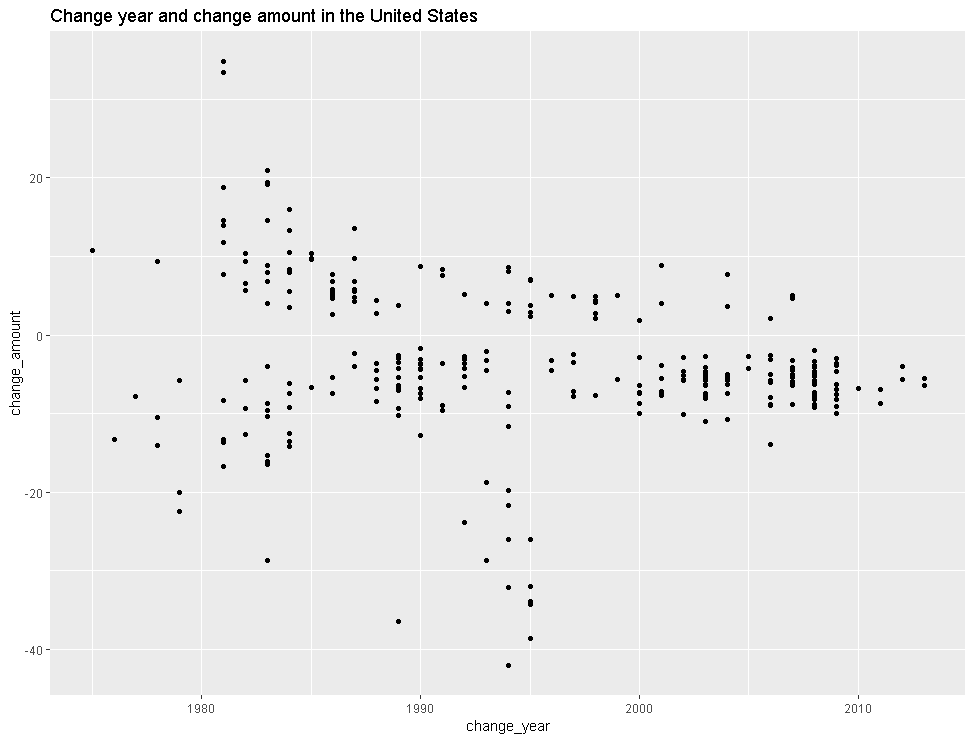
\includegraphics[width=0.7\linewidth]{plots/clustering/year_amount.png}
    \caption{Relationship between change amount and year in the United States}
    \label{year_amount}
\end{figure}

Looking at these plots, we see that most of the positive changes occurred before 1990 and all of the significant increases occur before 1985. We also see a cluster of large decreases in Southern California primarily occurring during the 1990s. Additionally, we see that after the year 2000 most of the changes that occur are slight decreases in the mean on the East Coast. To try and create more formal groupings for these change points, we decided to use clustering techniques on the change amount and year.

\subsection{K-Means}
For our cluster analysis, we chose to use k-means clustering on the change amount and year. The goal of this method is to cluster all of our change points into $k$ partitions, with each point belonging to the cluster with the closest change amount and year using the euclidean distance. As our first step, we needed to determine what value of $k$ is optimal for our dataset. To do so, we used the elbow method. This method attempts to determine the ``optimal" number of clusters by increasing the number of clusters and looking at how each additional cluster impacts the variation within the clusters. We can then find a range of potential values of $k$ based on when additional clusters don't reduce as much of the within cluster variation. The elbow plot for our method is included below. 

\begin{figure}[H] % vertical line for chosen cluster
    \centering
    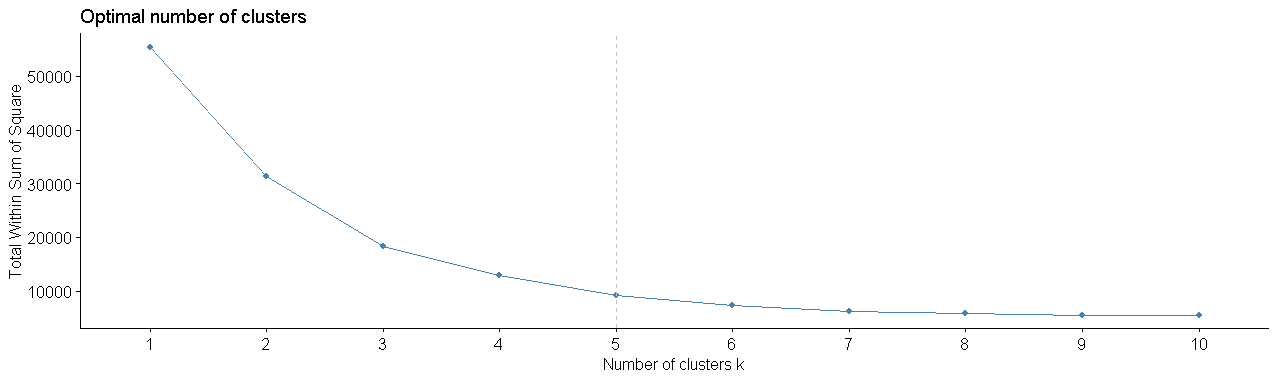
\includegraphics[width=\linewidth]{plots/clustering/elbow.png}
    \caption{Within cluster sum of squares for each potential cluster size.}
    \label{elbow}
\end{figure}

Using this plot, it was determined that the best number of clusters would be either 3, 4, or 5. To determine which number of clusters would be used, we examined the impact of the value of $k$ on the which points were clustered together and determined that $k=5$ would be used as it differentiated between the positive and negative changes after the year 2000. Having decided on a value of $k$, we then plotted examined the location of the clusters using both the year and amount.

\begin{figure}[H]
    \centering
    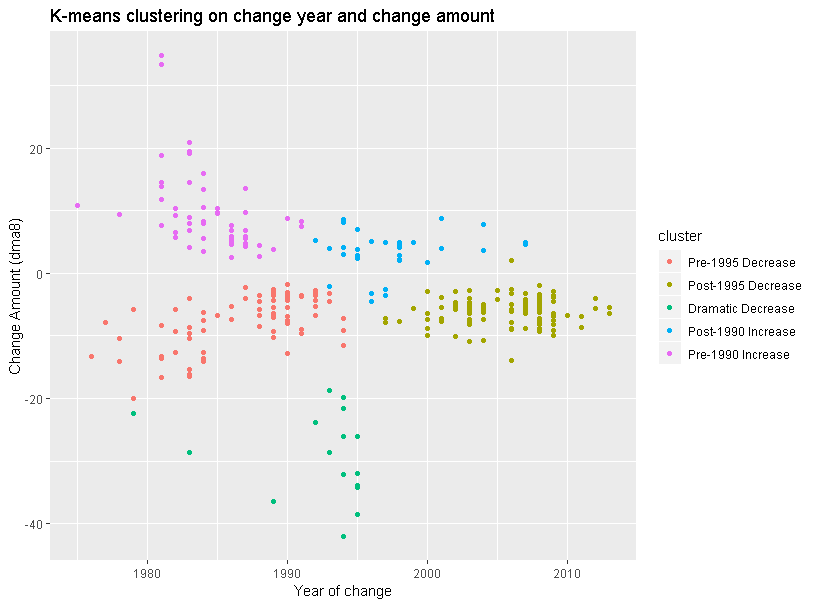
\includegraphics[width=0.7\linewidth]{plots/clustering/year_amount_clusters.png}
    \caption{K-means clusters for each station, change amount and year}
    \label{k_means}
\end{figure}

% typo
We named each cluster based on the direction of the change and the year that clusters are separated by. There are a few stations that don't follow the exact rules (points in the post-1990 increase clusters that had slight decreases) but as a general rule they represent the cluster. The final cluster was named ``Dramatic Decrease" as it represented all of the decreases over 20 ppb of dma8 levels across a variety of years. The cluster had a mean year of change of 1992 and all of the points in this cluster appear to be focusted between 1992 and 1995. The earlier clusters had more extreme behavior than the later clusters - the mean of the early increases was 9.86 ppb to the later 3.47, while the early decreases were -7.66 ppb to the later -6.12. We next examined the physical locations of these stations.

% table summarizing cluster

\begin{figure}[H]
    \centering
    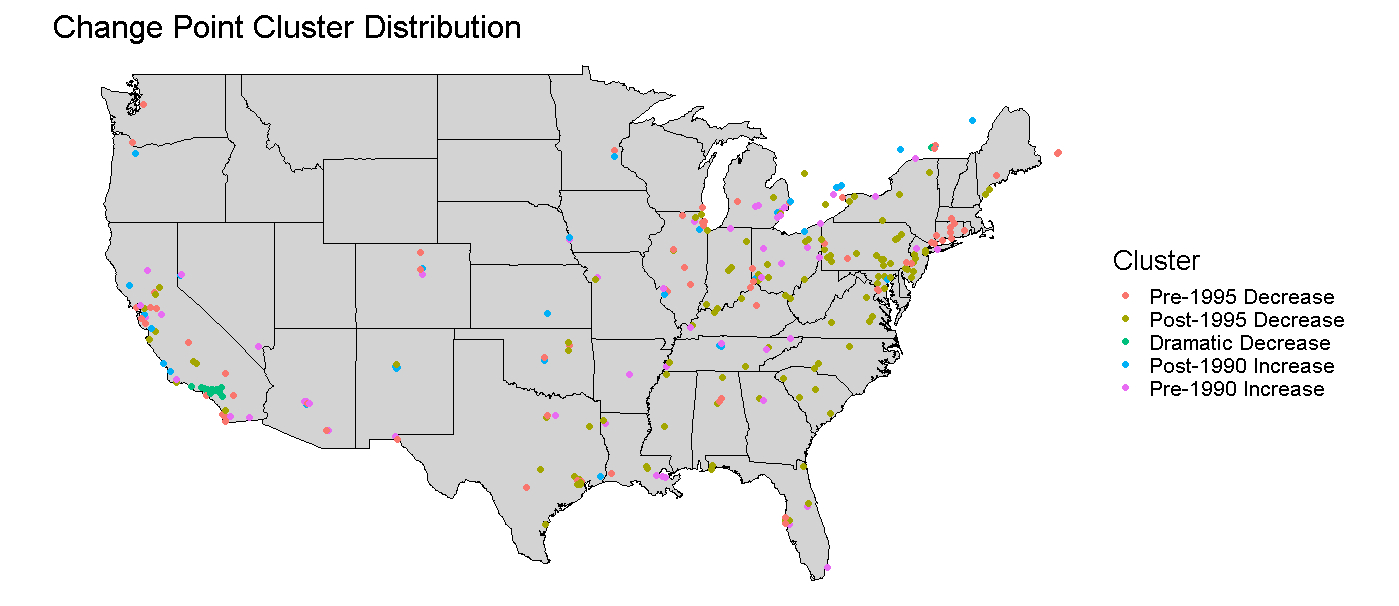
\includegraphics[width=\linewidth]{plots/clustering/spatial_cluster_all.png}
    \caption{K-means clusters for each station, geographic distribution}
    \label{k_means_geo}
\end{figure}

It's difficult to see if any of the clusters have any spatial relationship, so for clarity we examined each cluster individually. Below are two of these clusters (the stations with dramatic decreases and the post-1995 decreases) that appeared to have occurred in similar geographic areas. Using these plots we see that dramatic decrease seems to be focused in Southern California during the 1990's and the post-1995 decrease primarily across the Eastern U.S.

\begin{figure}[H]
    \centering
    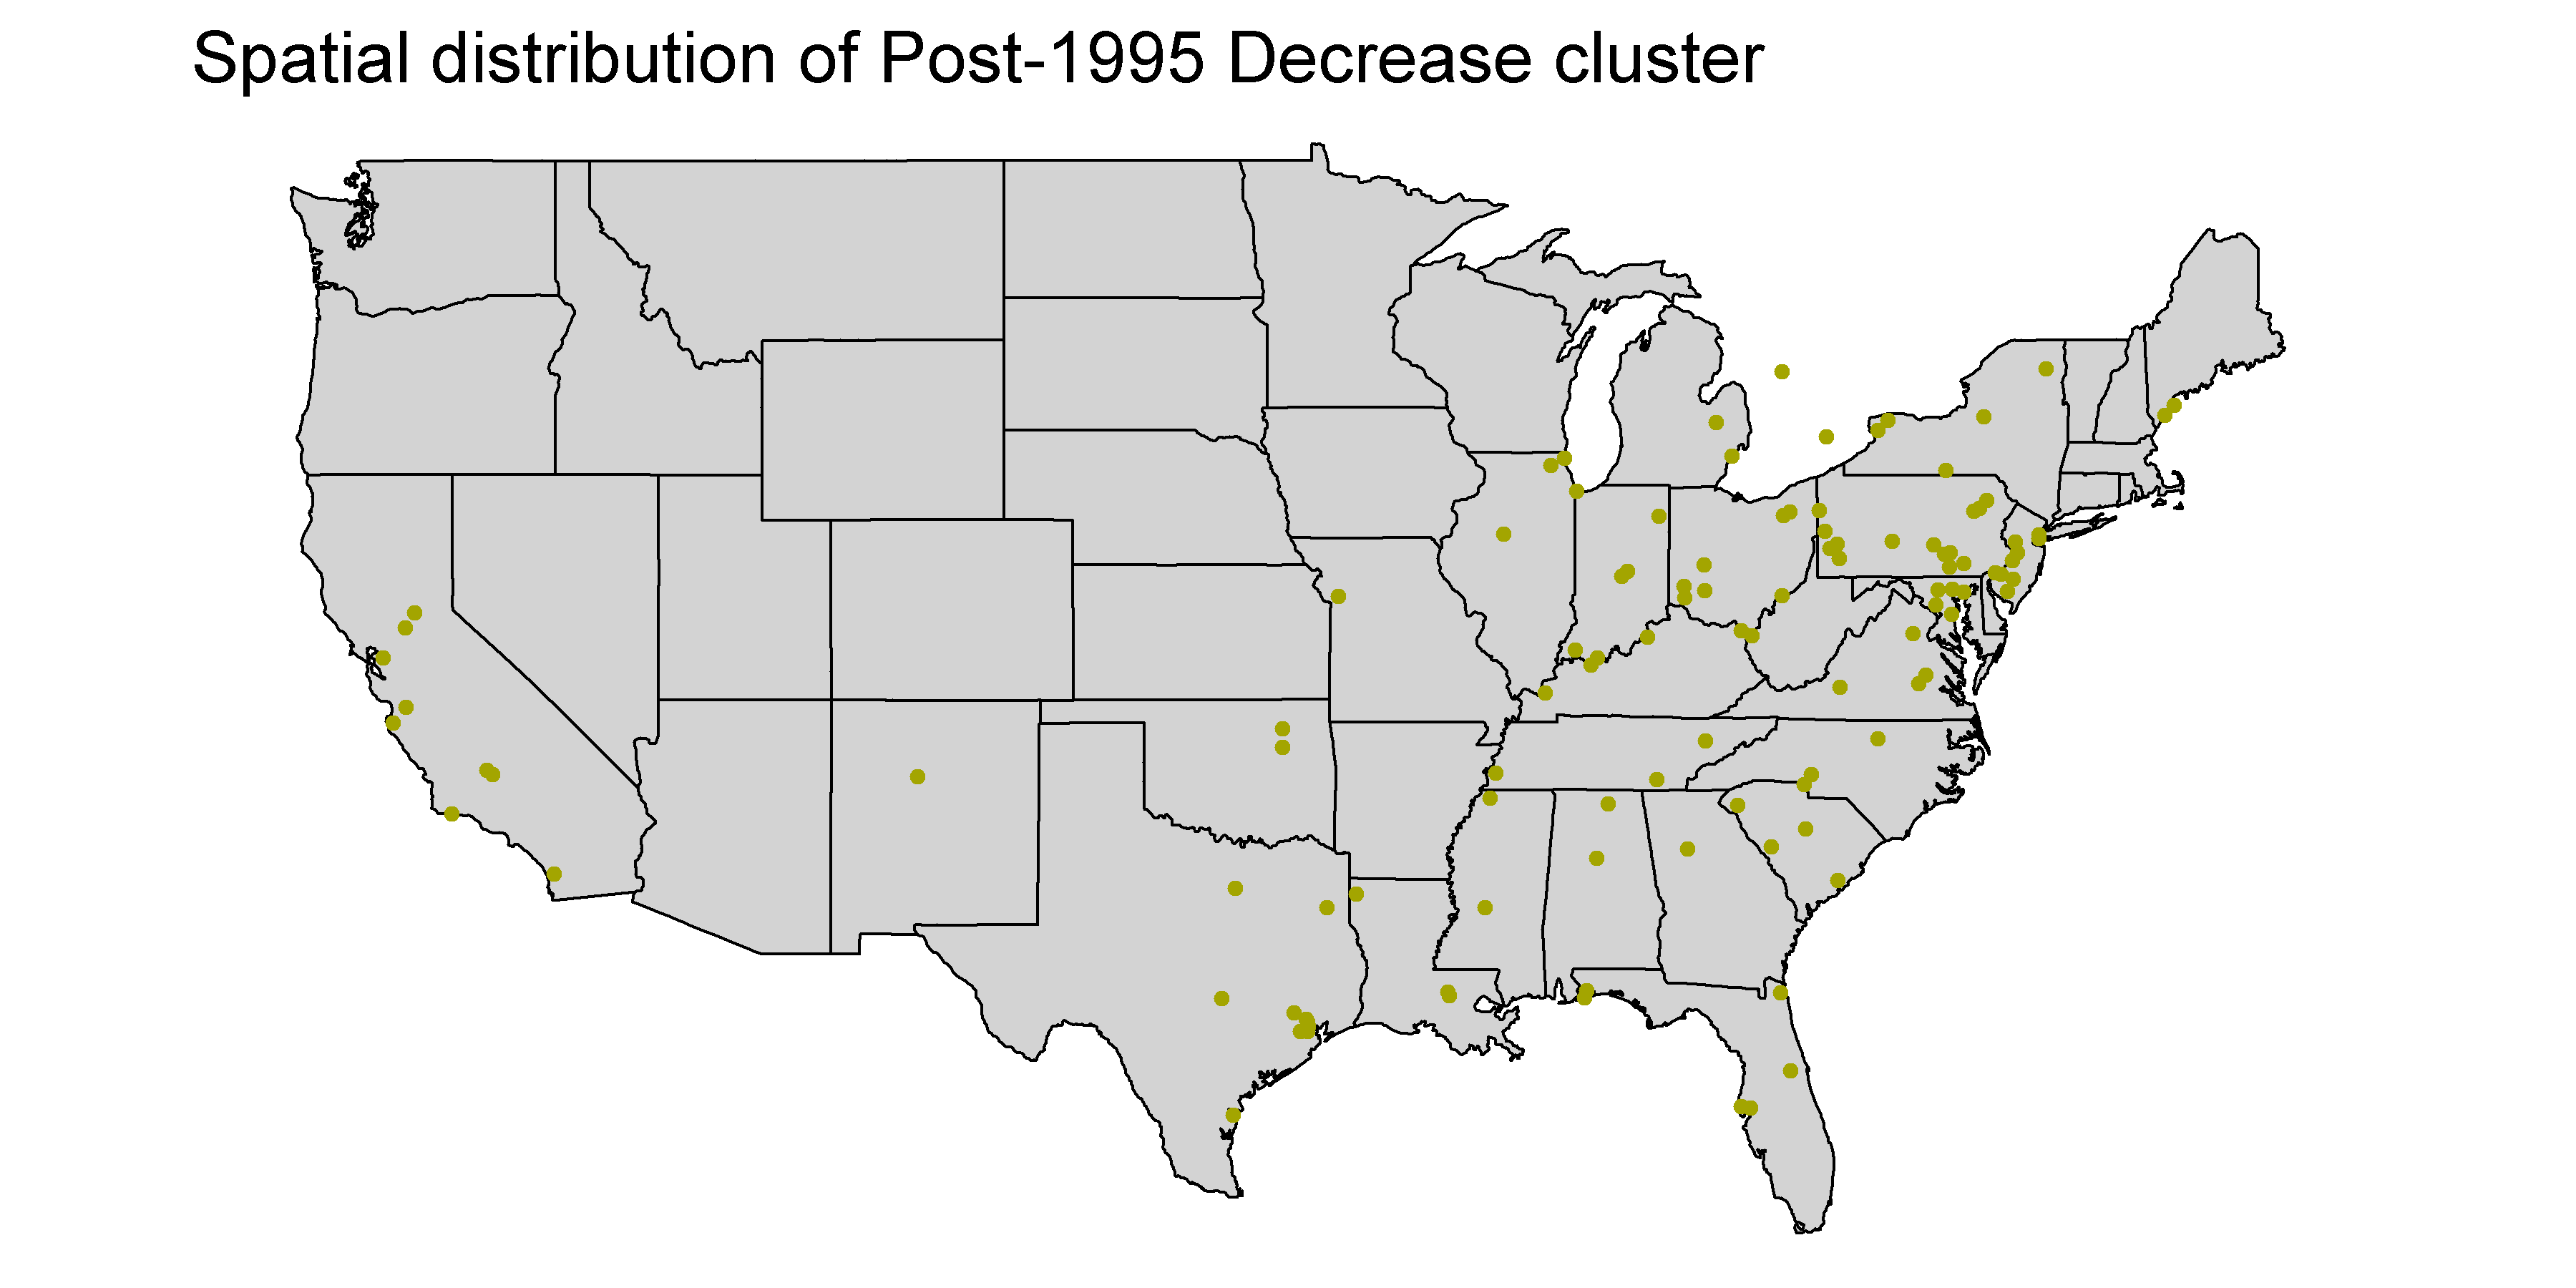
\includegraphics[width=0.9\linewidth]{plots/clustering/spatial_cluster_2.png}
    \caption{Spatial distribution of post-1995 decrease stations}
    \label{spatial_2}
\end{figure}

\begin{figure}[H]
    \centering
    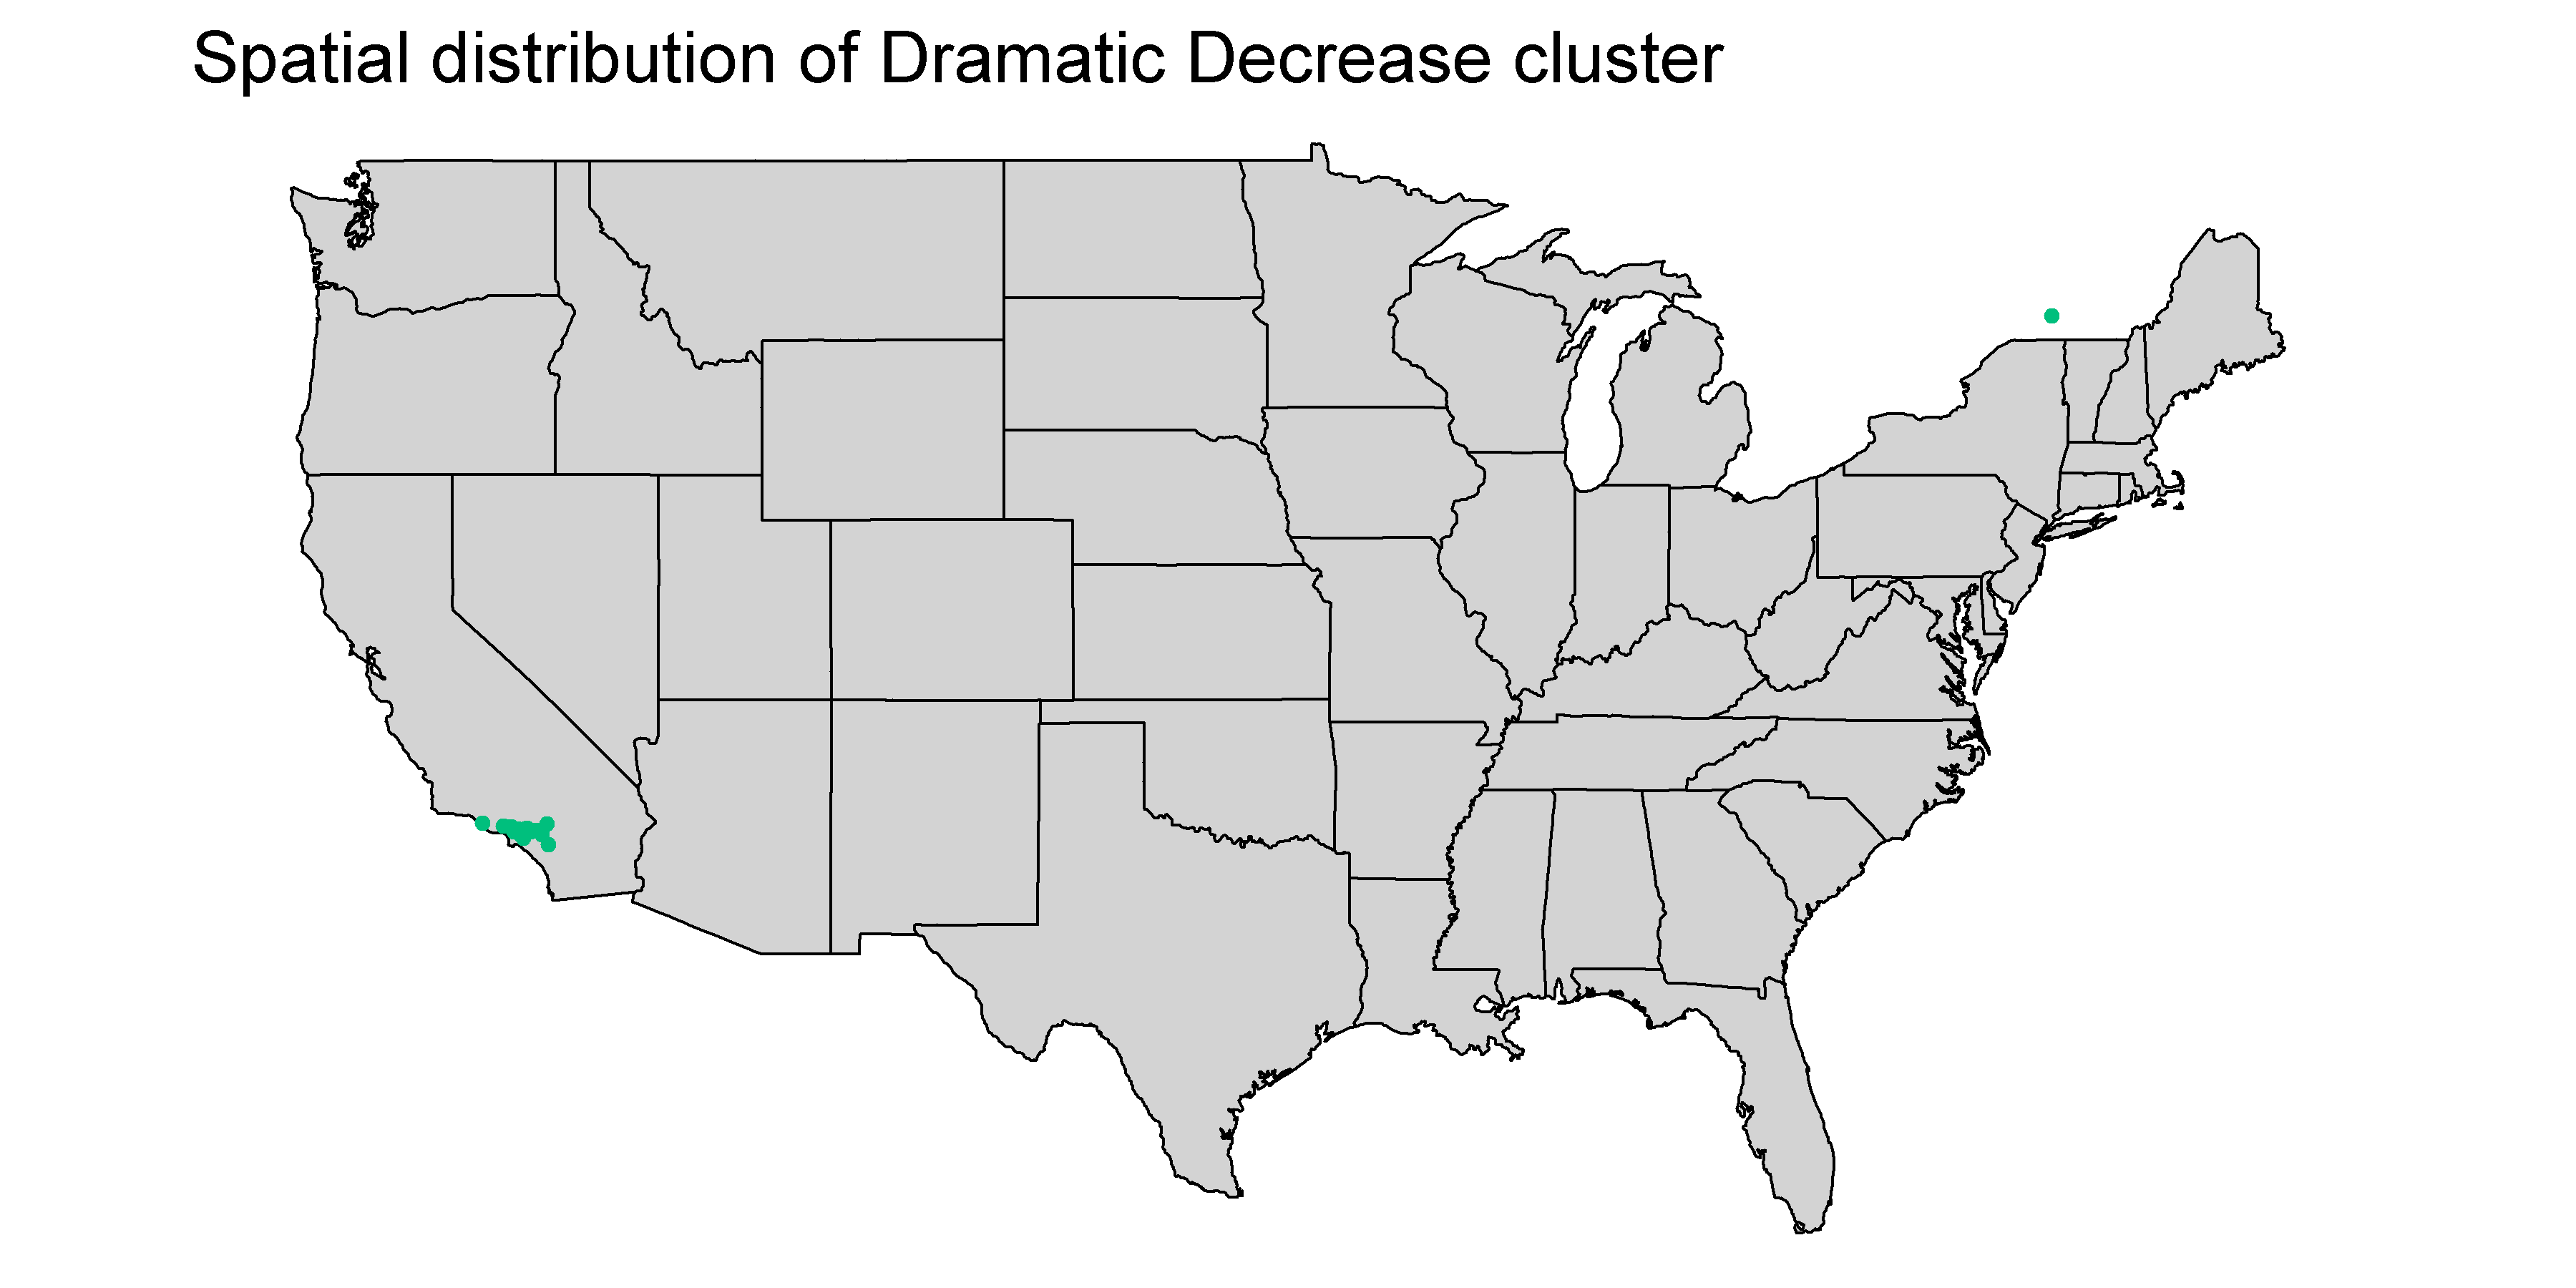
\includegraphics[width=0.9\linewidth]{plots/clustering/spatial_cluster_3.png}
    \caption{Spatial distribution of dramatically decreasing stations}
    \label{spatial_3}
\end{figure}

Additionally, we can use functional boxplots to examine how each cluster changes over time. In our case, these plots show information similar to traditional boxplots (the median, interquartile range, and outliers) but at each year. The plots are included below.

\begin{figure}[H]
    \centering
    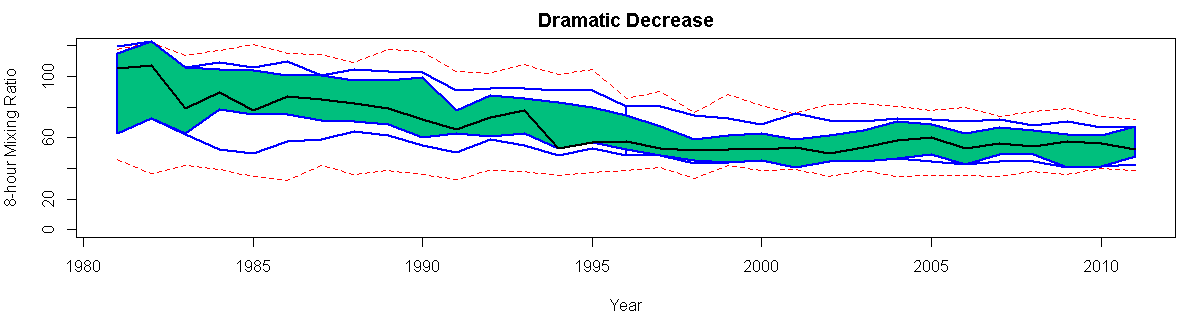
\includegraphics[width=0.9\linewidth]{plots/functional_boxplots/clust3.png}
    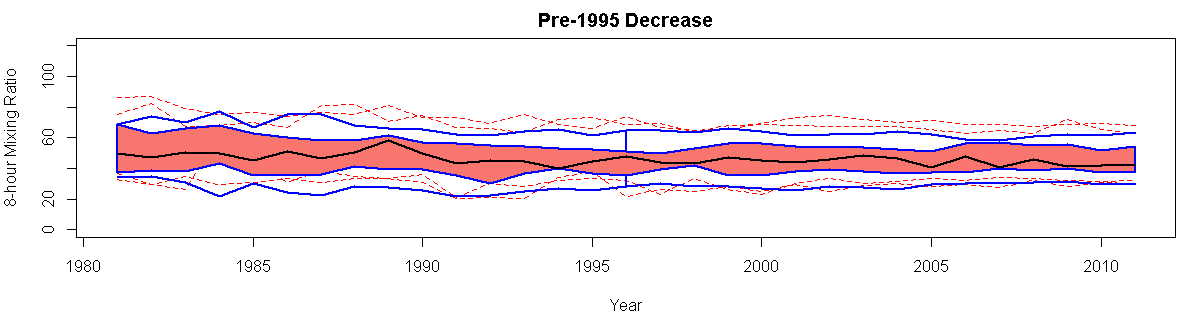
\includegraphics[width=0.9\linewidth]{plots/functional_boxplots/clust1.png}
    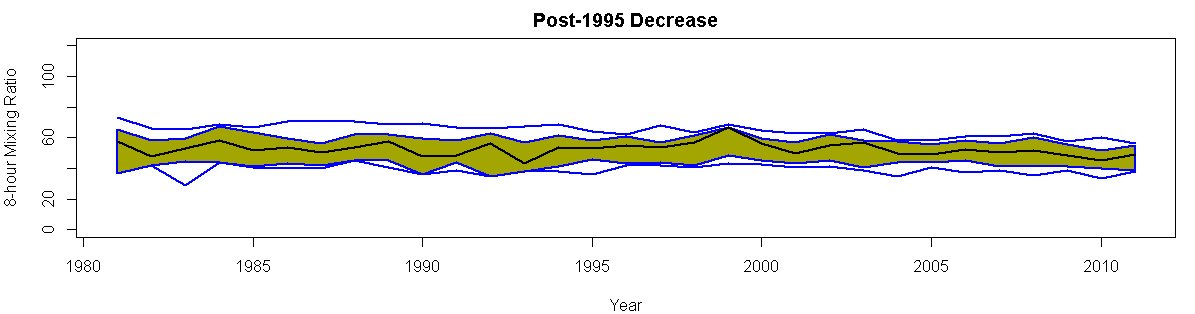
\includegraphics[width=0.9\linewidth]{plots/functional_boxplots/clust2.png}
\end{figure}
\begin{figure}[H]\ContinuedFloat
    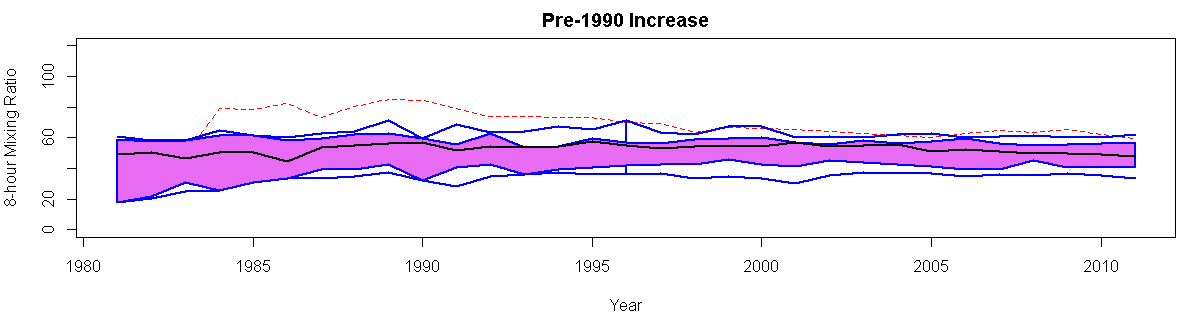
\includegraphics[width=0.9\linewidth]{plots/functional_boxplots/clust5.png}
    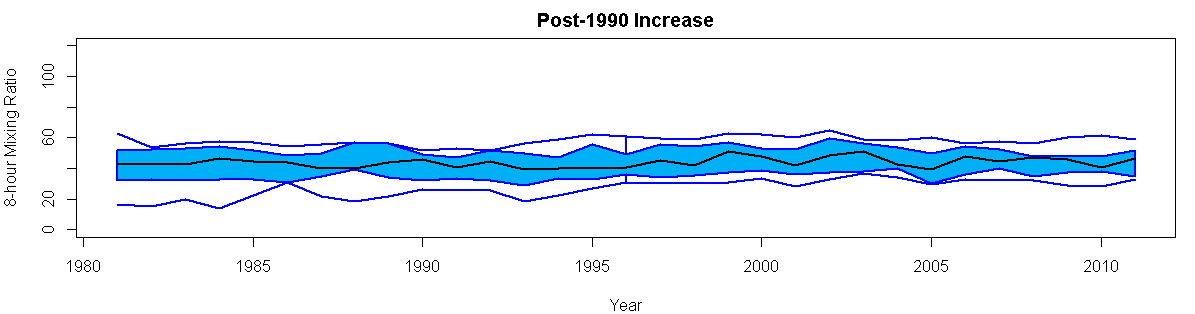
\includegraphics[width=0.9\linewidth]{plots/functional_boxplots/clust4.png}
    \caption{Functional boxplots for each cluster.}
    \label{fxn_box}
\end{figure}

The most dramatic effect demonstrated in these plots is the decline in dma8 values during the 1980s and 1990s for the cluster of dramatically decreasing means. Most of the other clusters don't appear to have any significant changes as a whole as their changes in mean weren't as large as those grouped into the dramatically decreasing cluster.

Next, we'll look closer at the areas during the two time periods discussed earlier (Southern California around 1995, Eastern U.S. after 2000) to examine what may have prompted these changes.

\section{Analysis of Area Specific Activity}
\subsection{Ohio Valley}
The Ohio Edison Company provides power for a large portion of the state of Ohio. In 1999 the Ohio Edison company was accused of violating the Clean Air Act, and in 2003 the U.S. District Court for the Southern District of Ohio confirmed that the company had failed to obtain Clean Air Act permits and install all required pollution controls for its plants. The settlement of the lawsuit filed by the United States and multiple nearby states included a major reduction of pollution from the power plants in question. Because of this we decided to explore ozone levels on the east coast of the United States. We hypothesized there would be a decrease in the ozone levels on the east coast due to the capping of emissions at the Ohio Edison power plants. A plot of the direction of change of mean levels of dma8 on the East Coast of the United States can be seen in Figure \ref{east_coast_direction} . 

\begin{figure}[H]
    \centering
    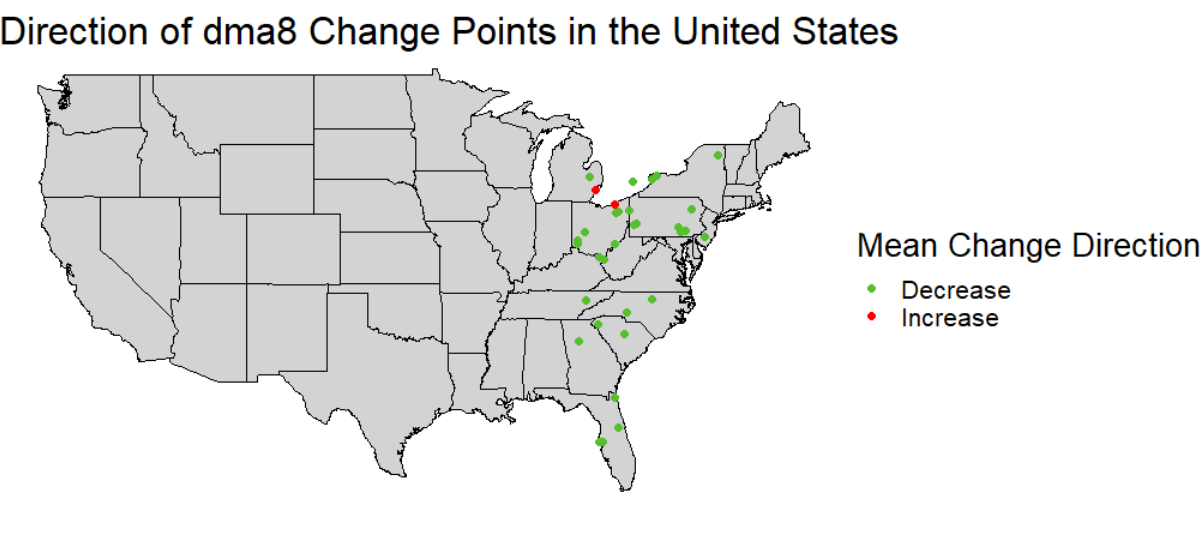
\includegraphics[width=0.8\linewidth]{plots/east_coast_direction.png}
    \caption{Direction of Change in Ozone on the East Coast}
    \label{east_coast_direction}
\end{figure}

Of 33 stations located on the east coast that had a change point after 2005, 31 had a decrease in mean ozone levels while 2 had an increase. Therefore 93.9\%\ of stations located in the eastern United States had a decrease in ozone levels. This affirms our hypothesis that most stations on the east coast would see a decrease in ozone levels after the Ohio Edison was required to reduce emissions, however this is most likely not the only reason that the majority of stations had a decrease in ozone levels. The two stations that did not have a decrease in ozone levels are located in northern Ohio and south eastern Michigan relatively close together, but they are both north of all other stations located in Ohio which could explain why the decrease in emissions did not cause their mean ozone levels to drop. The capping of emissions for the Ohio Edison company most likely had an effect on the ozone levels at some stations on the east coast, but other factors and decreases in air pollutants could also explain these decreases.

\subsection{Southern California}
From our clusters, we found that there was a dramatic decrease in the levels of ozone in Southern California during the early to mid 1990's. Los Angeles is an interesting example of a major city, because it relies primarily on private transportation rather than public transportation that is widely adopted in other major cities such as New York or Chicago. This causes larger amounts of auto emissions. During the time before the 1984 Olympics, which took place in Los Angeles, Southern California adopted strict measures to "reduce both
vehicle and industrial emissions [which] resulted in significantly cleaner air during the Olympics" (\cite{parrish_xu_croes_shao_2016}). The cleaner air experienced during the Olympics caused a lasting impact on pollution measures in Southern California which can explain the large decrease in Ozone amounts in the 10 years after they hosted. An example of one time series plot from the Southern California area is shown \ref{socal_ts}

\begin{figure}[H]
    \centering
    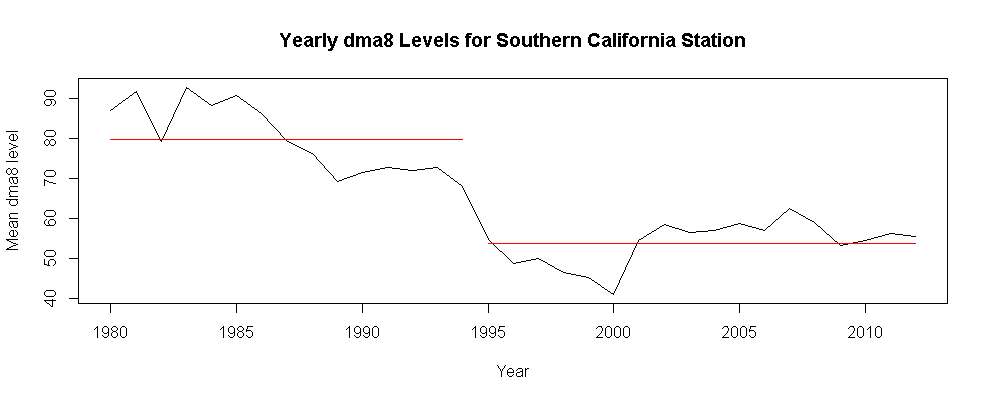
\includegraphics[width=1\linewidth]{plots/time_series/socal_example.png}
    \caption{Southern California Time Series Plot}
    \label{socal_ts}
\end{figure}

If you look at the time series shown in \ref{socal_ts}, there is a large dip in ozone levels around 1984 when the Olympics took place. There is a small increase after that year, however the levels then decrease dramatically starting in 1985 until a change point in the mean ozone level occurs in 1995. The stringent pollution regulations put into place are most likely the cause of this dramatic decrease in the ozone levels in Southern California cluster. 

\section{Conclusion}
During our research we looked at change points in the mean dm8 levels of ozone in the United States. The time and level at which these change points occurred is important for examining how ozone trends are behaving over time. Within our work we clustered on the time and level of change points which also proved interesting results. The clustering analysis resulted in 5 different clusters: pre-1995 decrease,post-1995 decrease, dramatic decrease, post-1990 increase, and pre-1990 increase. After our clustering analysis we decided to focus on 2 specific areas where changes in mean dm8 levels of ozone occurred. The first area we focused on was all stations on the east coast that had a change point after 2005. We concluded that a large contributor to this was a change in power plant activity in the Ohio Valley. The second area we focused on was the dramatic decrease cluster. This cluster is comprised of almost only stations located in Southern California. Because of this spatial factor we decided this cluster needed a more in depth analysis. This cluster all had change points in the early to mid 1990's, which is only a few years after Los Angeles implemented strict anti-pollution and emission laws to increase air quality when the city hosted the Olympics. After the Olympics the city decided to continue these practices which is most likely a factor in the dramatic decrease in mean dm8 levels of ozone. 


\subsection{Future Work}
There are several areas of analysis that could be focused on during future work. The first would be to expand our work from being solely USA based to other areas of the world. One issue surrounding this is that most other areas of the world do not have data ranging back for 25 years, so future work in this area may require waiting for more data to become available. Another area of future exploration would be to implement the same change point and clustering analysis we did on the AMOC method to the PELT method. This would require more fine tuning of the PELT method to make sure the change points detected are valuable, but could also result in new findings not shown with the AMOC method. 

\newpage
 
\section{Previous Analysis}
The below research and analysis is from previous work on this data. Our original research goal was to make connections between extreme ozone events and economic factors. The initial analysis did not show promising results, so we decided to change the scope of our project and research goal. The work done on the original research goal can be found below.
\subsection{Introduction}
\subsubsection{Research Goal} % worth expanding
Our overall research goal is to find connections between extreme ozone events and economic trends and growth. We hope to outline how extreme ozone events have moved throughout time to areas where economic growth is more prominent. This will hopefully outline the relationship between growth and extreme ozone events. 

\subsubsection{Data}
The data we are going to use will come from the TOAR database (\cite{schultz2017apmd}). The variables we have decided to use to classify an extreme ozone event are the number of days above 70 ppb and the average daily maximum 8-hour average ozone mixing ratios. The number of days above 70 ppb will allow for identification of location specific extreme events that occur occasionally, while the daily maximum mixing ratios will allow us to explore the long term exposure and effects of ozone. 

 We will examine the real GDP for each country as our indicator for economic trends. This data was obtained from the World Bank. We could also use state or city level data in the United States, as the large area tends to mask trends within the country (such as the different behaviour in the southwest and northeast). By getting more discrete data, we should be able to create more accurate models. An example of this could be the state and city level GDP data provided by the U.S. Bureau of Economic Analysis.


\subsection{Statistical Methods}

For our initial model exploration, we created standard linear models relating GDP and year to the various emissions metrics. These models did not show a linear relationship between the GDP and emissions metrics. This could potentially be because while the GDP growth of poorer nations may cause large increases in emissions, growth in wealthier nations may result in wider use of clean energy.  We could potentially examine the relationships between the changes in GDP and emissions metrics rather than the metrics themselves to create a more convincing model. In addition, we could examine using other types of model (such as a generalized linear model) or looking at transformations of our metrics.

Because the relationship between GDP and extreme ozone events did not appear to be normal, we decided to explore using a generalized linear model. A generalized linear model is useful in modeling a linear relationship between data that does not follow the normal distribution. To begin we decided to model one station in Japan using a generalized linear model with a Poisson family. 

In addition to these linear models, we have considered performing cluster analysis on the data. In our cluster analysis, we would hope to visualize where the most extreme events happen and examine any trends in this movement.




\subsection{Findings}
\subsubsection{Initial Findings}
Figure 1 is plot of the $99^{th}$ percentile ozone levels in North America. In this plot we can see the general distribution of pollution across the US and Canada as well as the extreme levels at the location with in Mexico. Figure 2 shows the relationship between real GDP and the daily maximum 8-hour mixing ratios. Each point in this plot represents these values for a certain country in a certain year (e.g. Mexico in 2004). 

%\begin{figure}[ht]
%    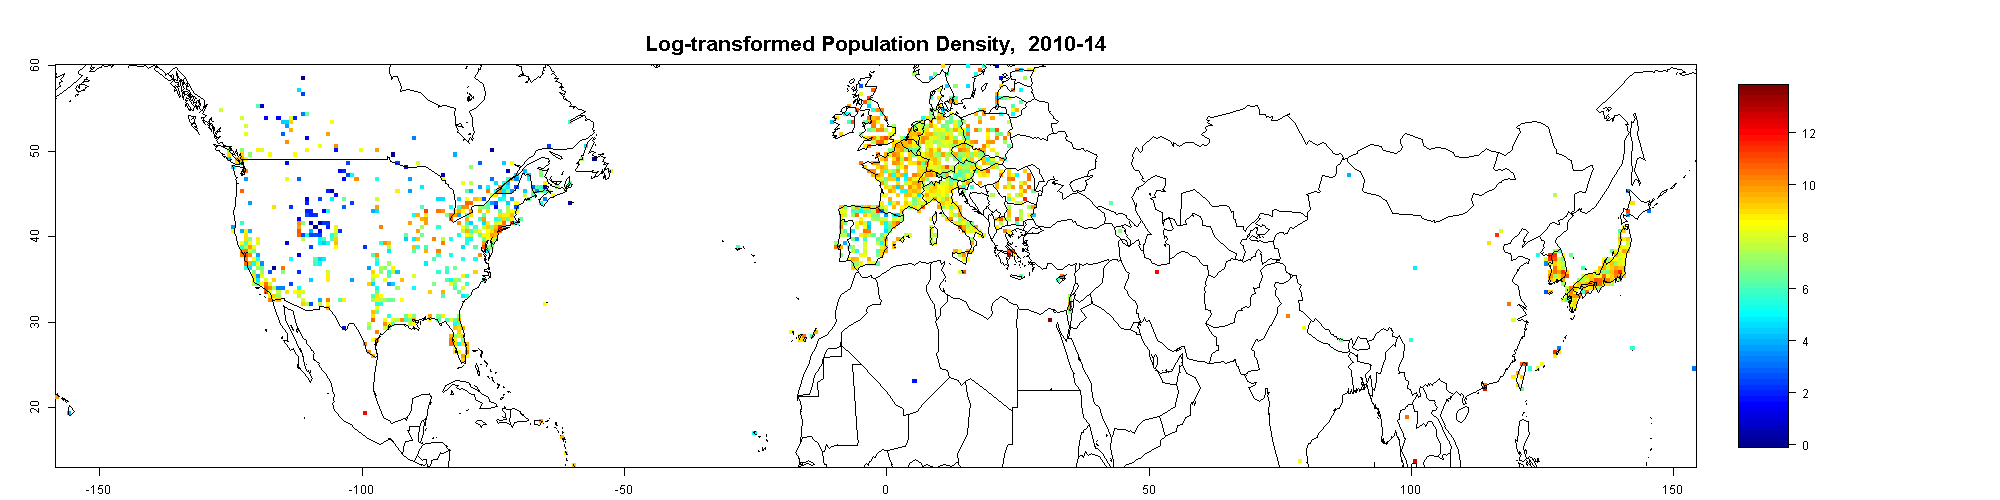
\includegraphics[width=\linewidth]{plots/population_2010-14.png}
%    \caption{Aggregated population density from 2010-2014 at station according to GPW version 3.}
%    \label{fig:population}
%\end{figure}

%\begin{figure}[ht]
%    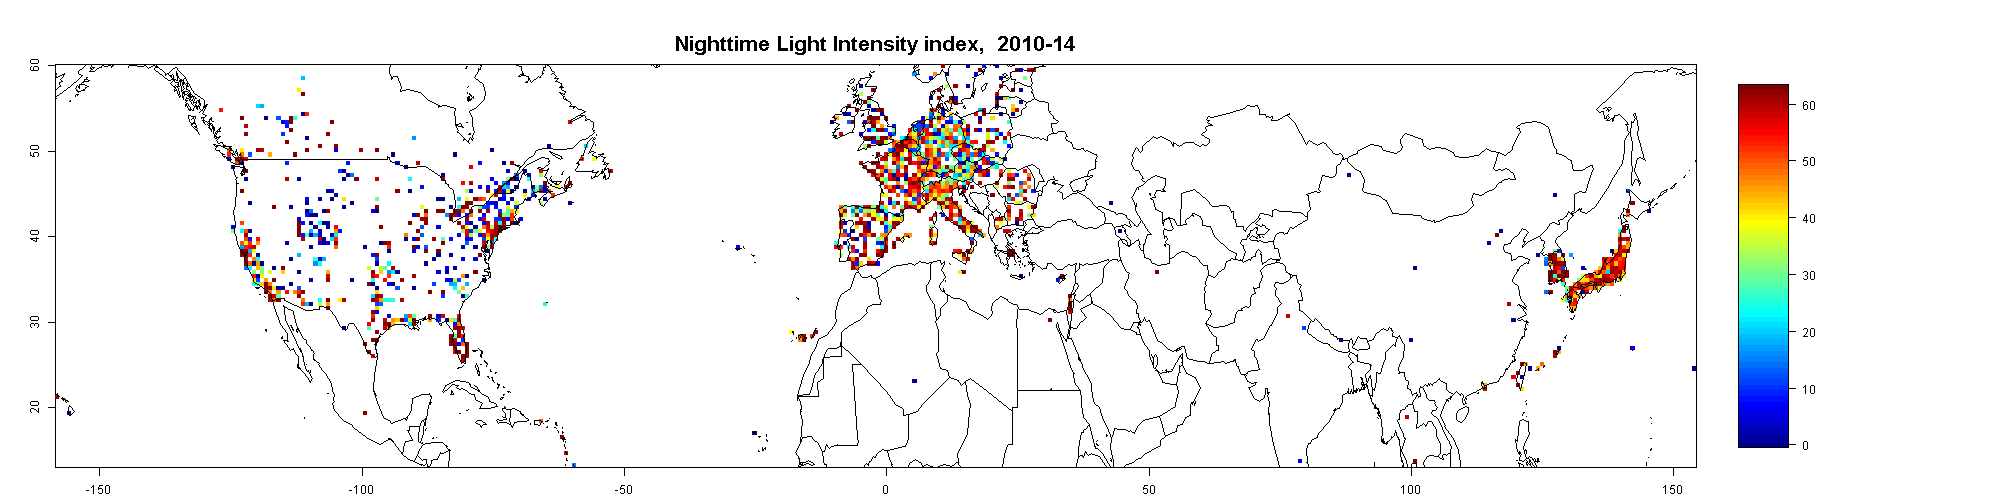
\includegraphics[width=\linewidth]{plots/lights_2010-14.png}
%    \caption{Nighttime light intensity index from 2010-2014 from NOAA-DMSP.}
%    \label{fig:lights}
%\end{figure}

\begin{figure}[ht]
    \centering
    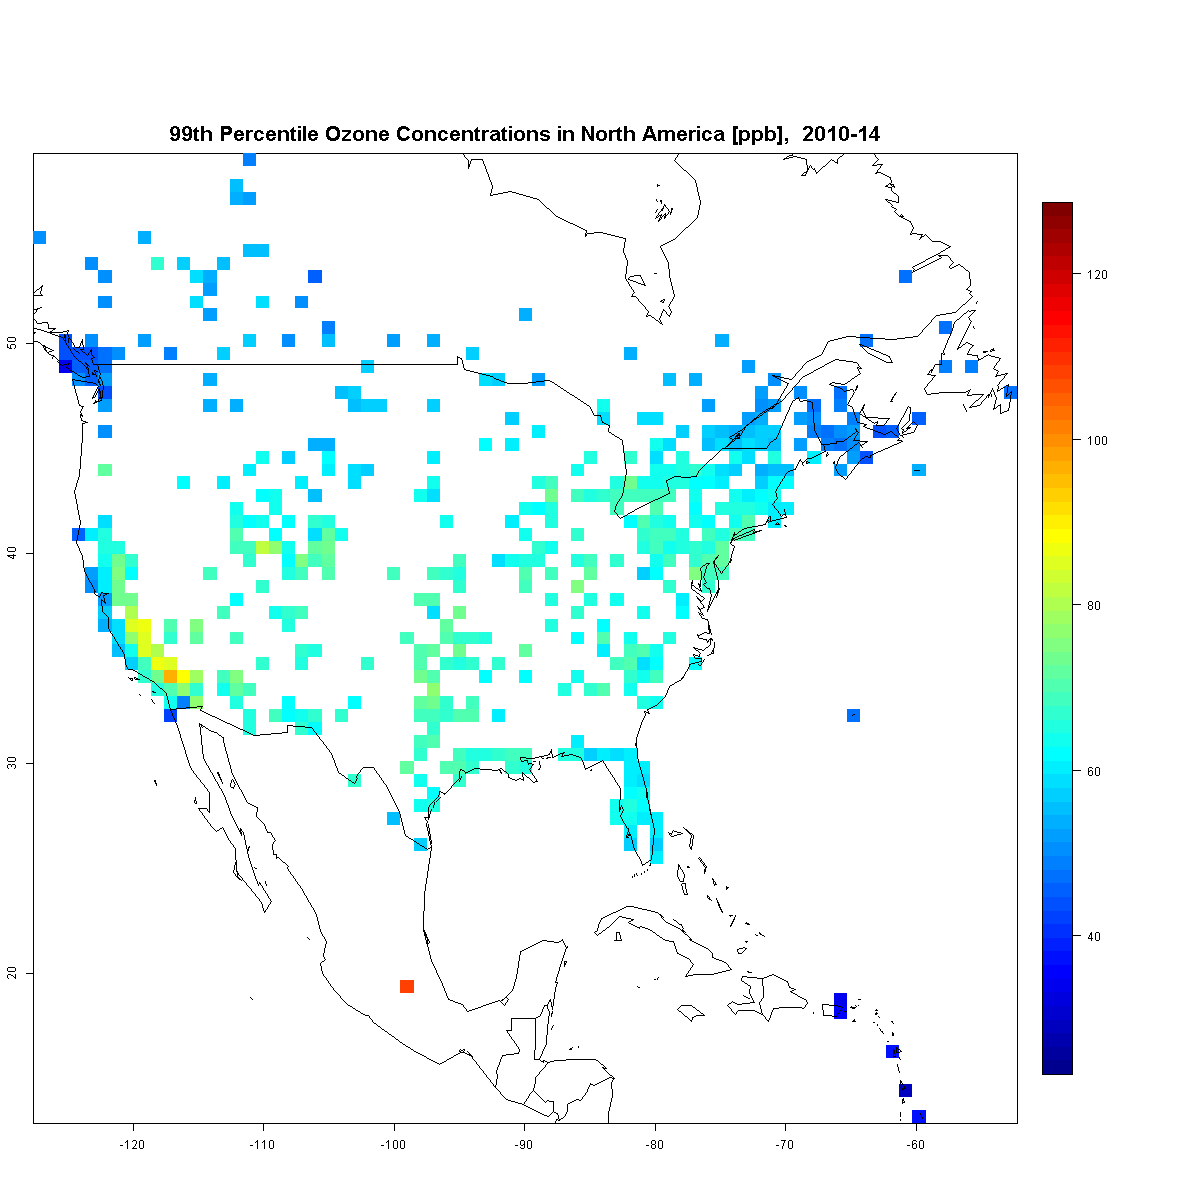
\includegraphics[width=0.5\linewidth]{plots/na_2010-14.png}
    \caption{Aggregated $99^{th}$ percentile ozone levels from 2010-2014 for stations in North America.}
    \label{fig:na}
\end{figure}

\begin{figure}[ht]
    \centering
    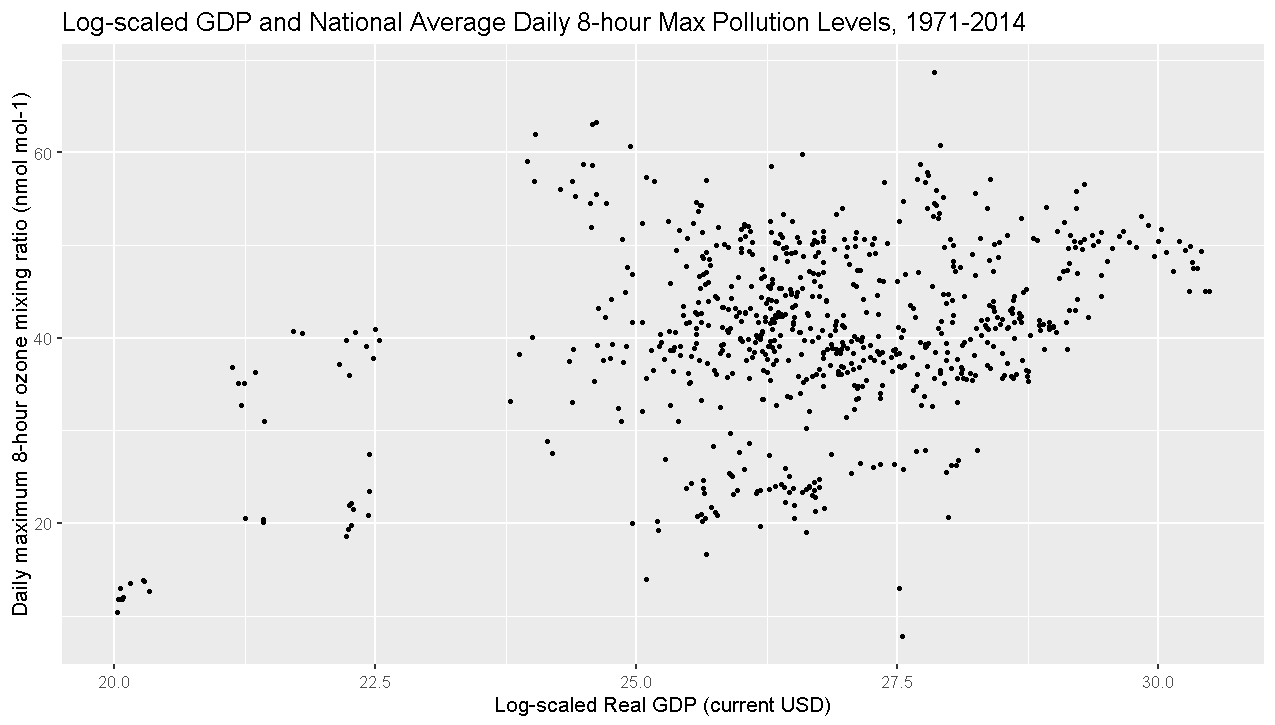
\includegraphics[width=0.6\linewidth]{plots/gdp_vs_dma8.png}
    \caption{Relationship between log-scaled GDP and the average 8-hour max ozone mixing ratio.}
    \label{fig:na}
\end{figure}

\newpage

\subsubsection{Generalized Linear Model}
To further try to represent the relationship between extreme ozone events and GDP, a generalized linear model was made. This model was made using the Days Over 70ppb at the Yamada station in Japan and the overall country GDP data. The generalized linear model created was generated using a Poisson distribution due to the Days Over 70ppb being a count of a certain number of events in a designated time period. An initial plot of the data is shown below in Figure 3. From the plot of the data it is unclear as to whether or not a Poisson generalized linear model will be able to describe the relationship between GDP and extreme ozone events. 

\begin{figure}[ht]
    \centering
    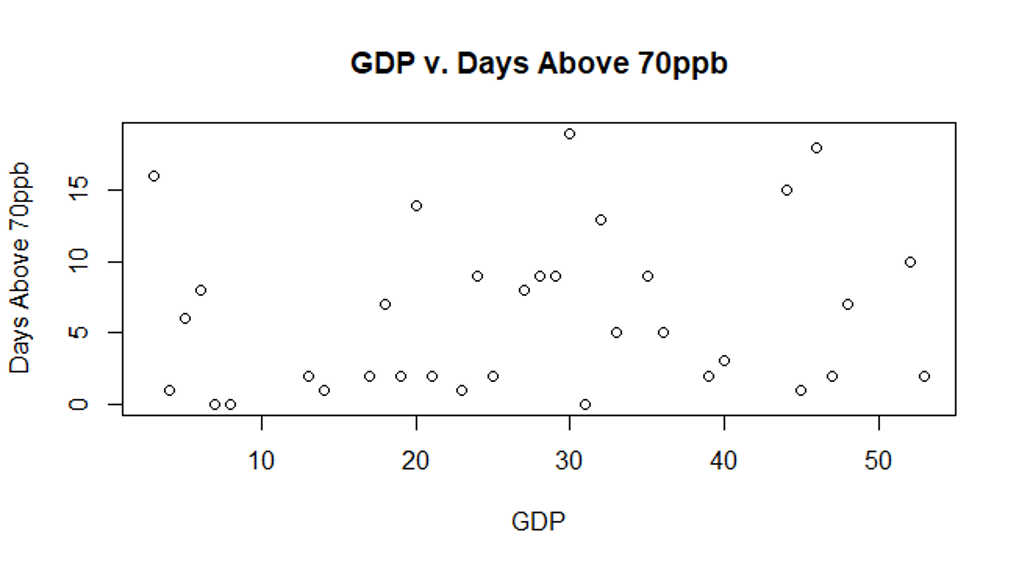
\includegraphics[width=0.7\linewidth]{plots/gdp_vs_days_above_70ppb.png}
    \caption{Days Above 70ppb in Yamada vs. Japan GDP}
    \label{fig:na}
\end{figure}

After the model was created, the ability of GDP in predicting the Days Above 70ppb for a certain year was not significant. This leads us to believe that a Poisson generalized linear model is not useful for describing the relationship between GDP and extreme ozone events on a country level for Japan.
We come to the conclusion that one type of generalized linear model, or standard linear model will not be useful in describing worldwide trends and that models will have to be developed on a country by country basis. 


\subsubsection{GDP and Extreme Ozone Events Time Series} % bad title will change
To better understand the relationship between GDP and extreme ozone events we created explanatory plots from time series data in four countries. Below are the plots and analyses for relationship between GDP and the 8 Hour Daily Average and GDP and Days Over 70ppb for Germany, Japan, Spain, and the United States. In our plots, we decided to display the ozone metrics as a moving average as it helped smooth the data and make it easier to interpret.

\newpage

\begin{figure}[ht]
    \centering
    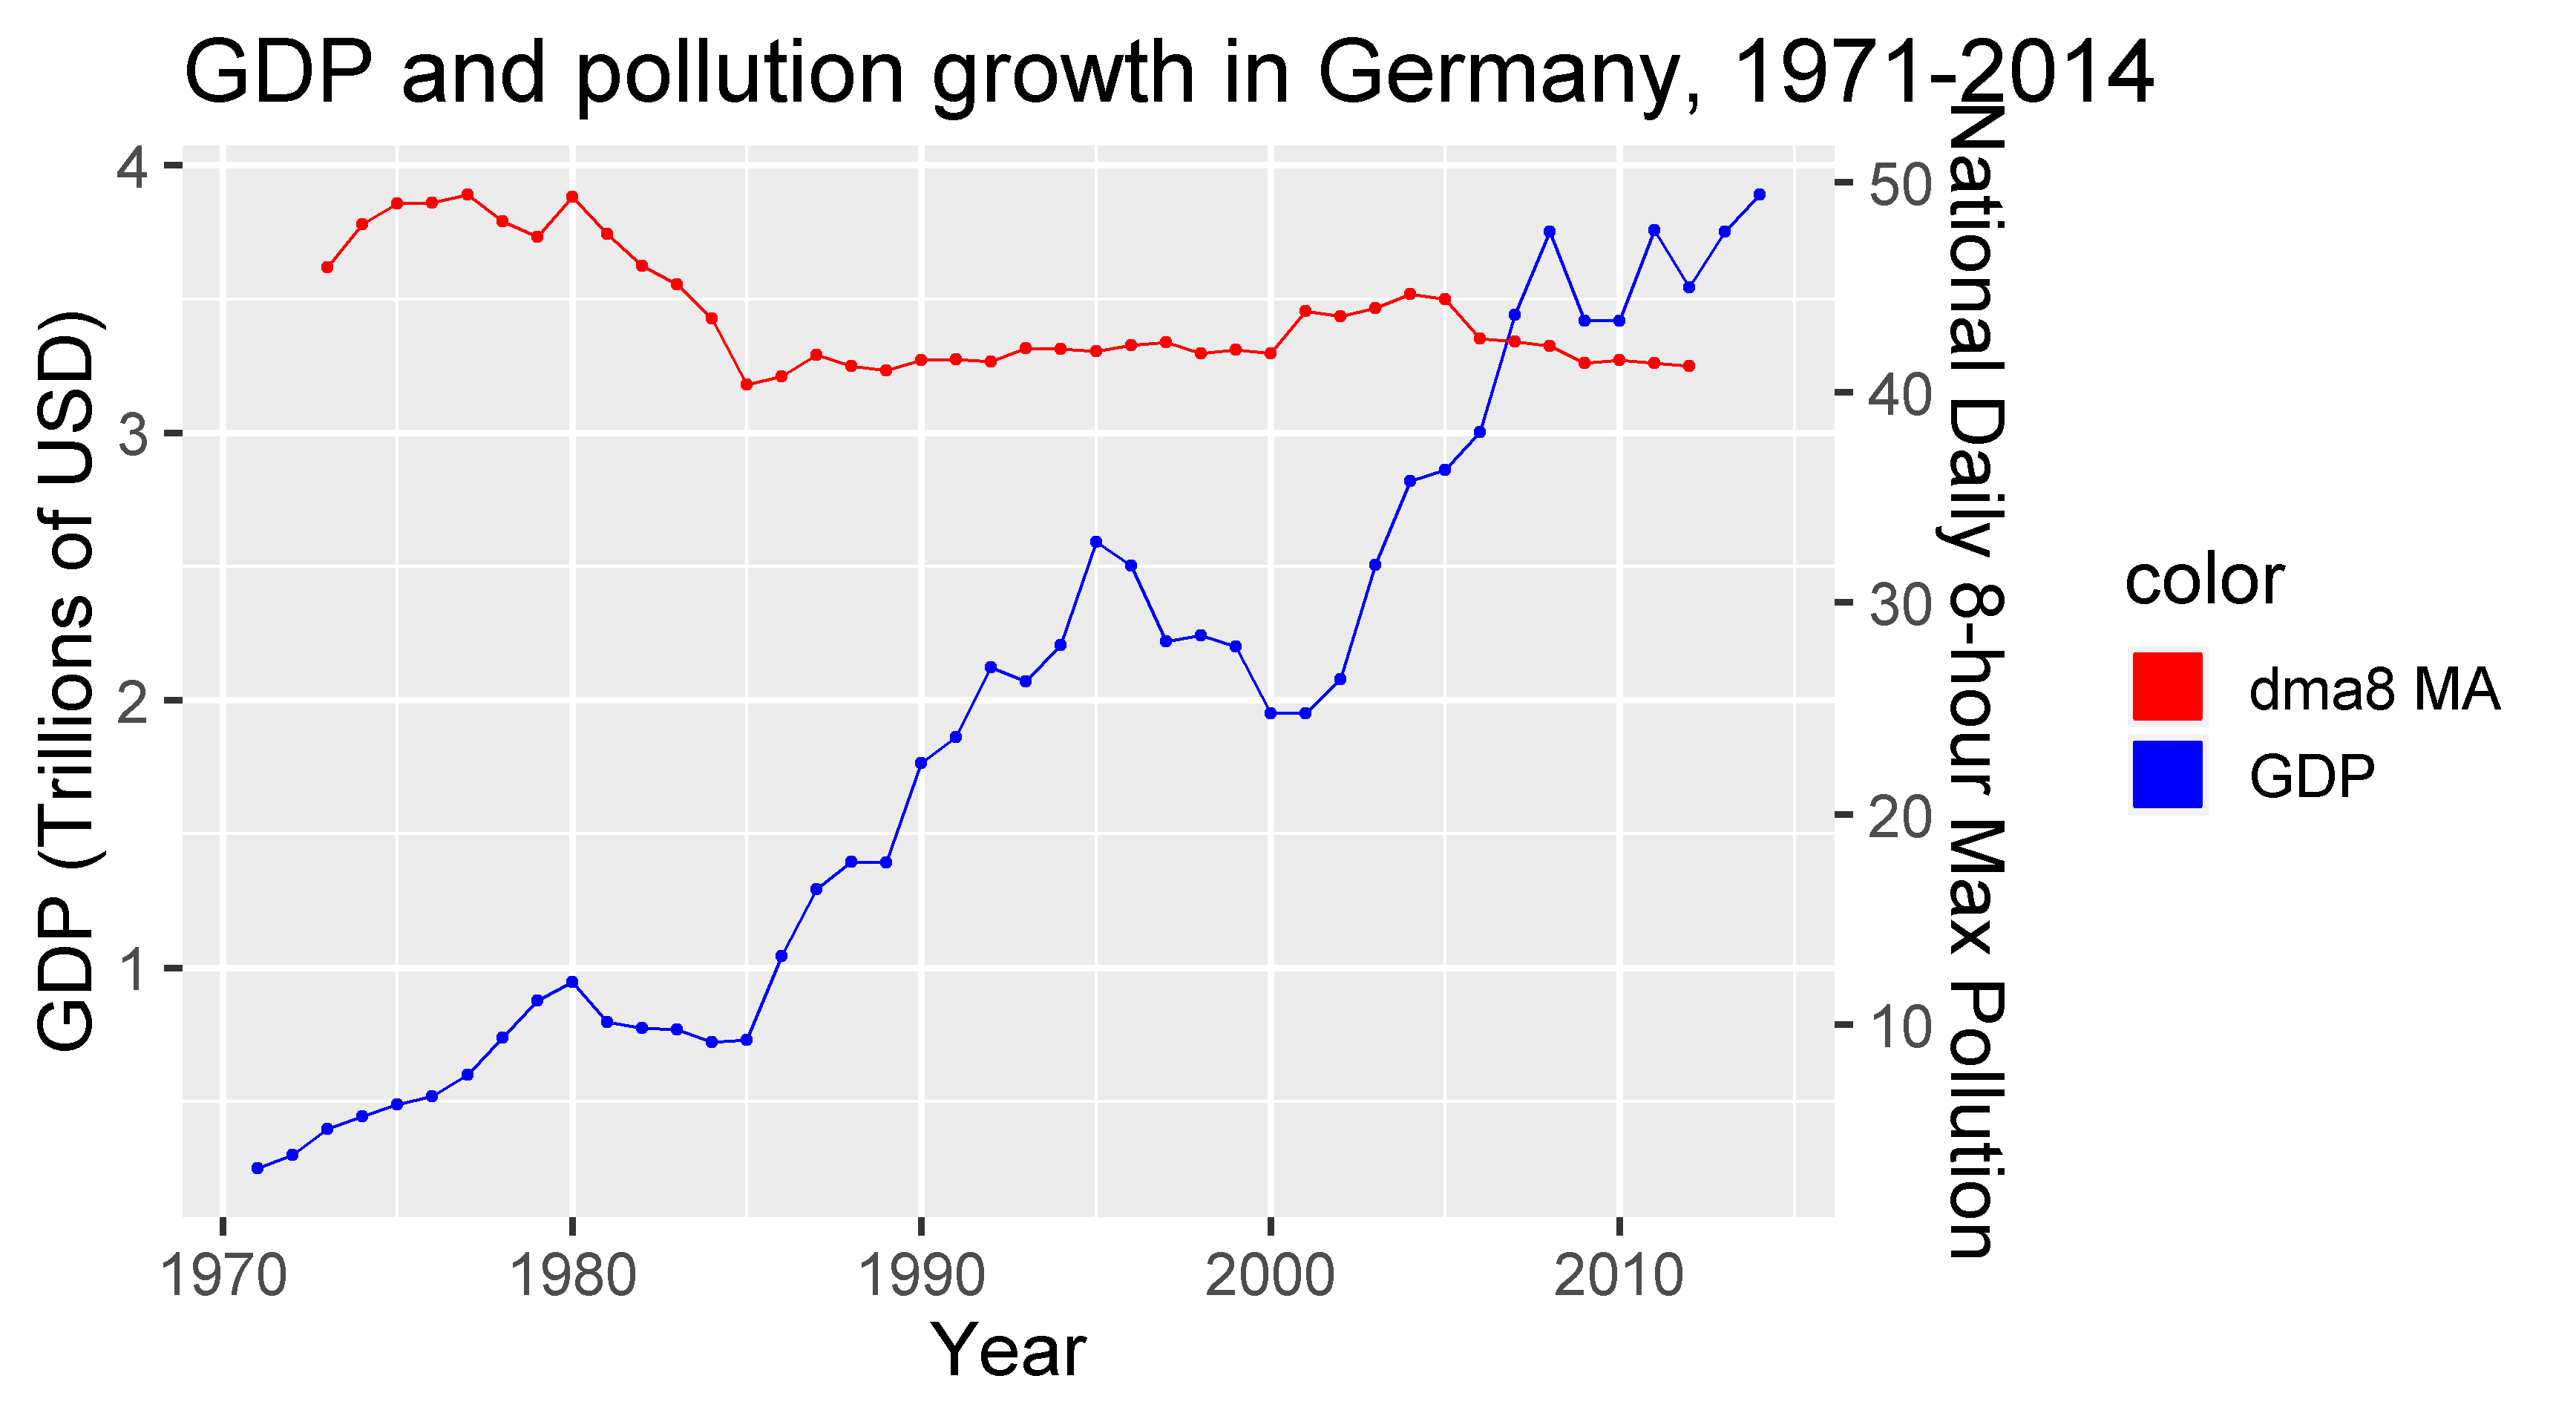
\includegraphics[width=0.45\linewidth]{plots/country_pollution/Germany_dma8.png}
    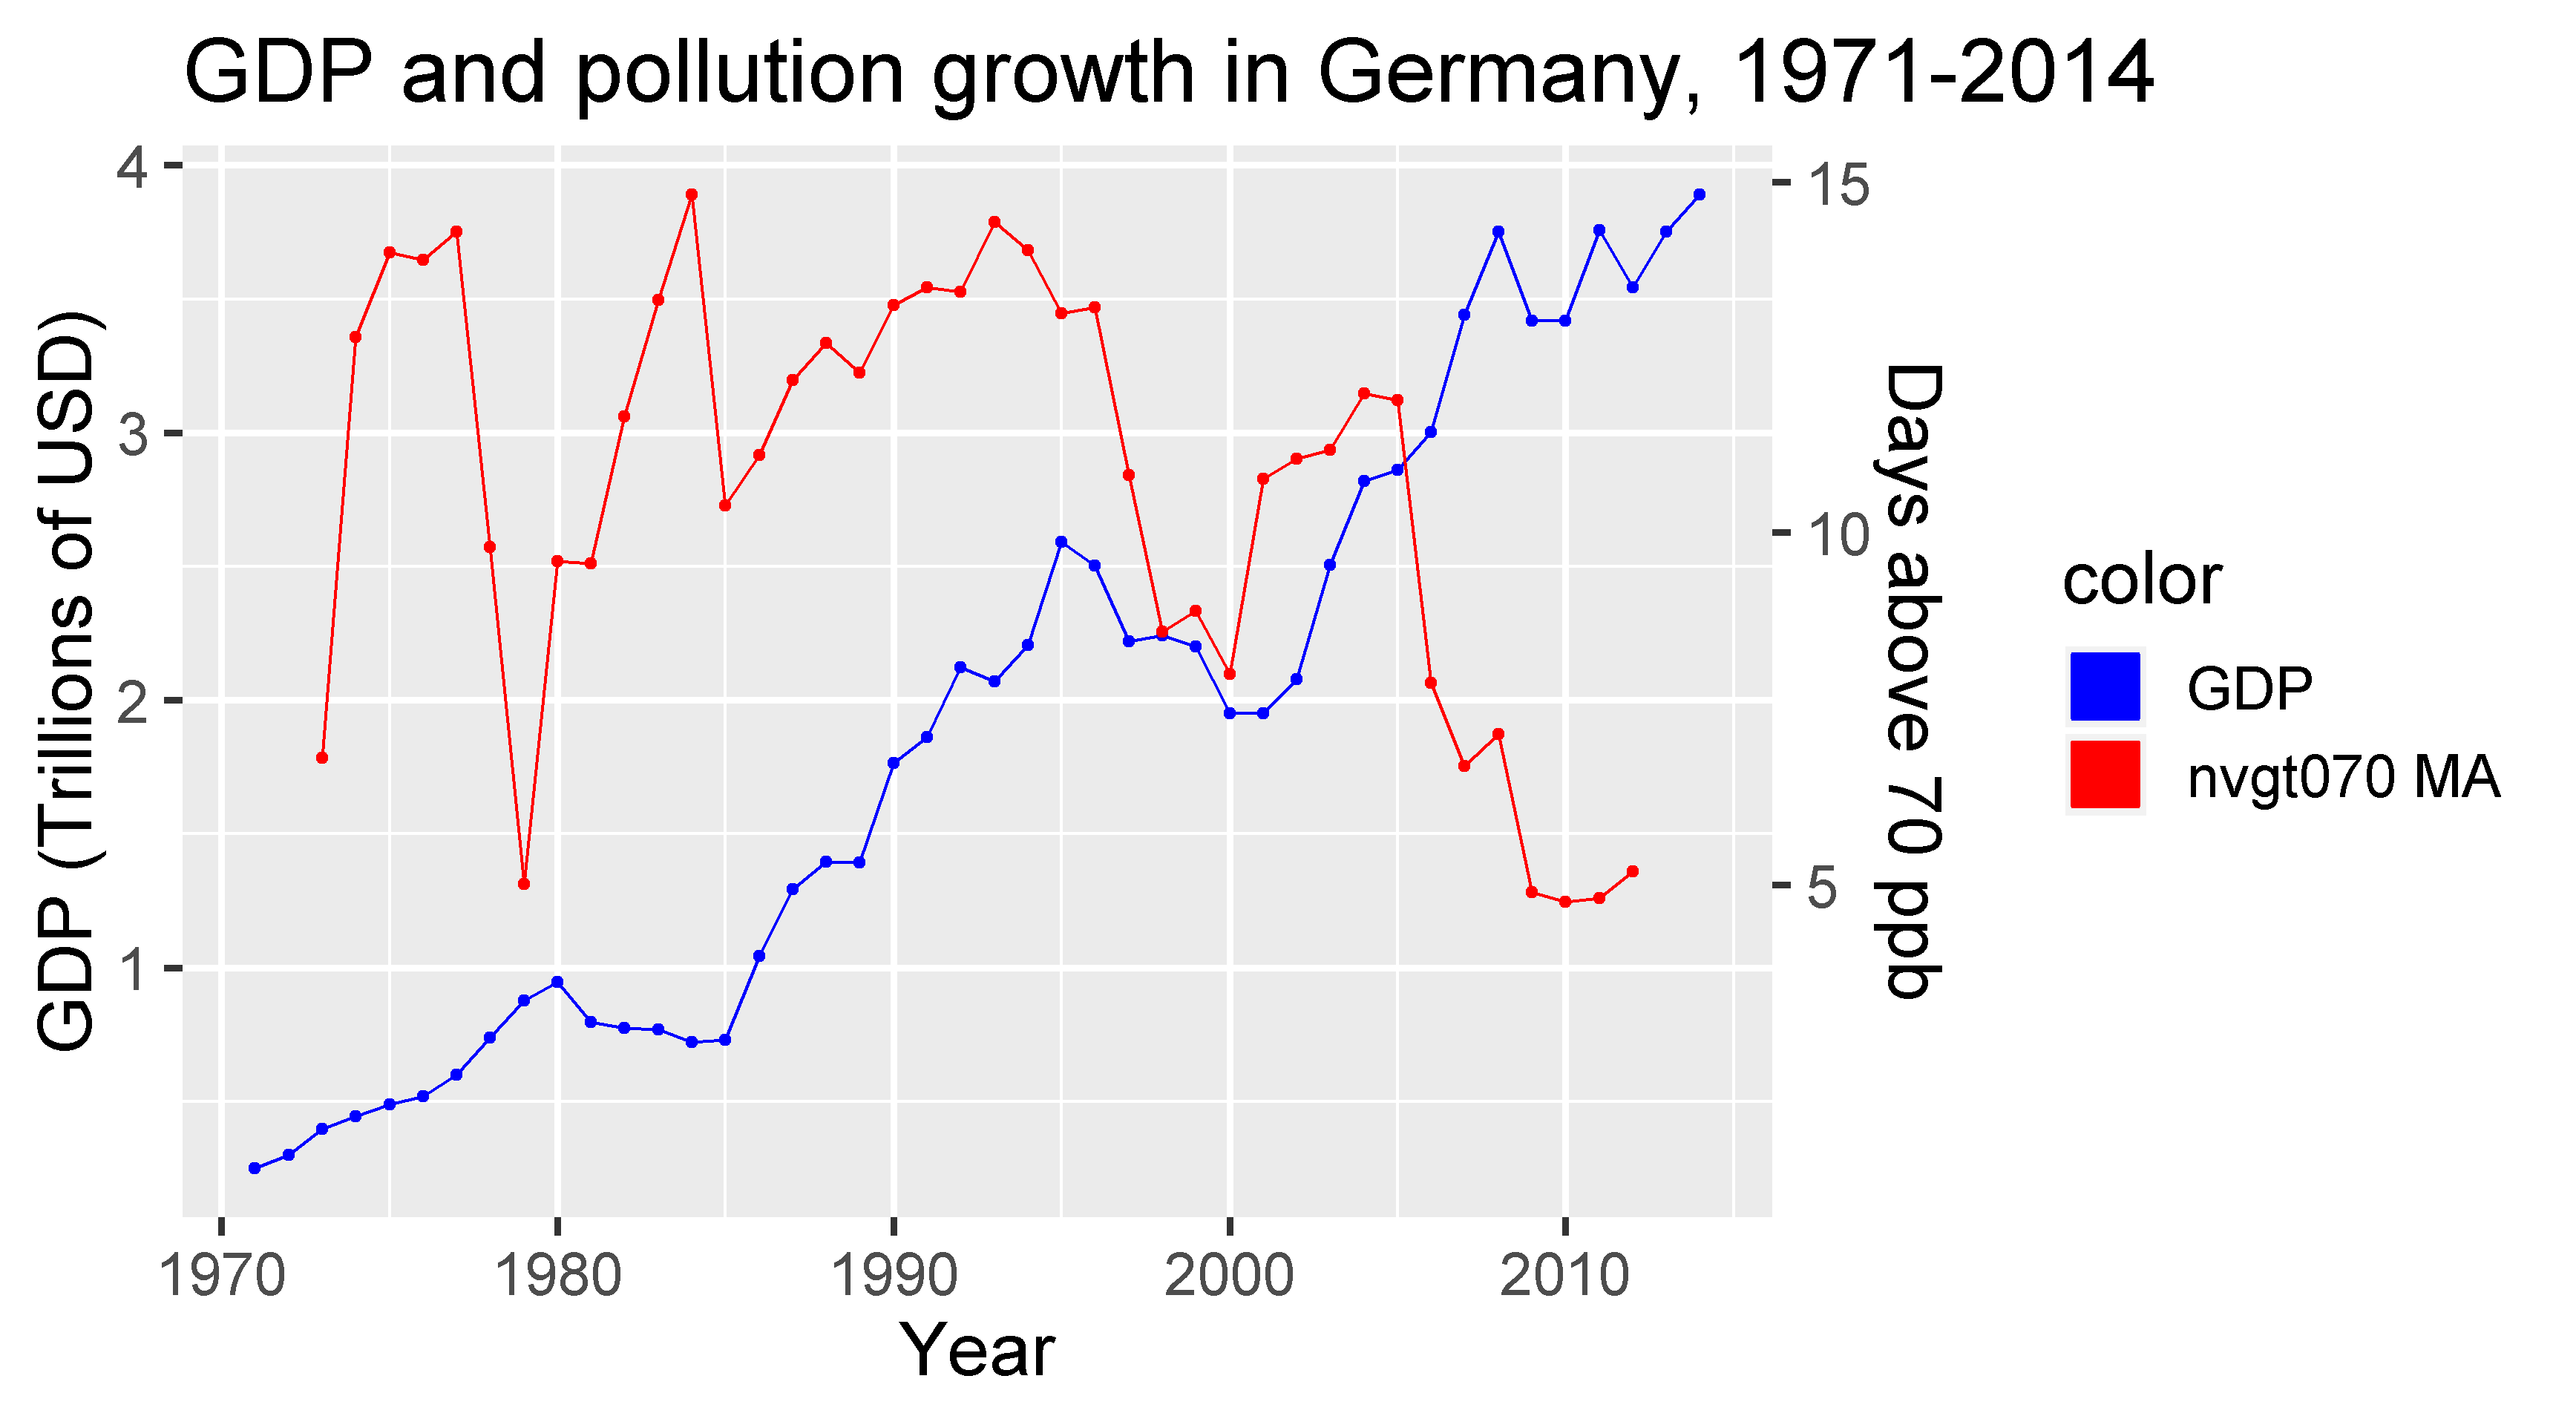
\includegraphics[width=0.45\linewidth]{plots/country_pollution/Germany_nvgt.png}
    %\caption{Germany}
    \label{fig:GER}
\end{figure}

In these plots, we can see that since 1971 Germany's economy has risen at a fairly consistent rate. We see that the days above 70ppb tended to be larger before the year 1995 and smaller afterwords, while the mixing ratios declined through the 1970's and 80's and were fairly constant afterwords. These ozone metrics don't appear to have a strong relationship with the GDP levels.

\begin{figure}[ht]
    \centering
    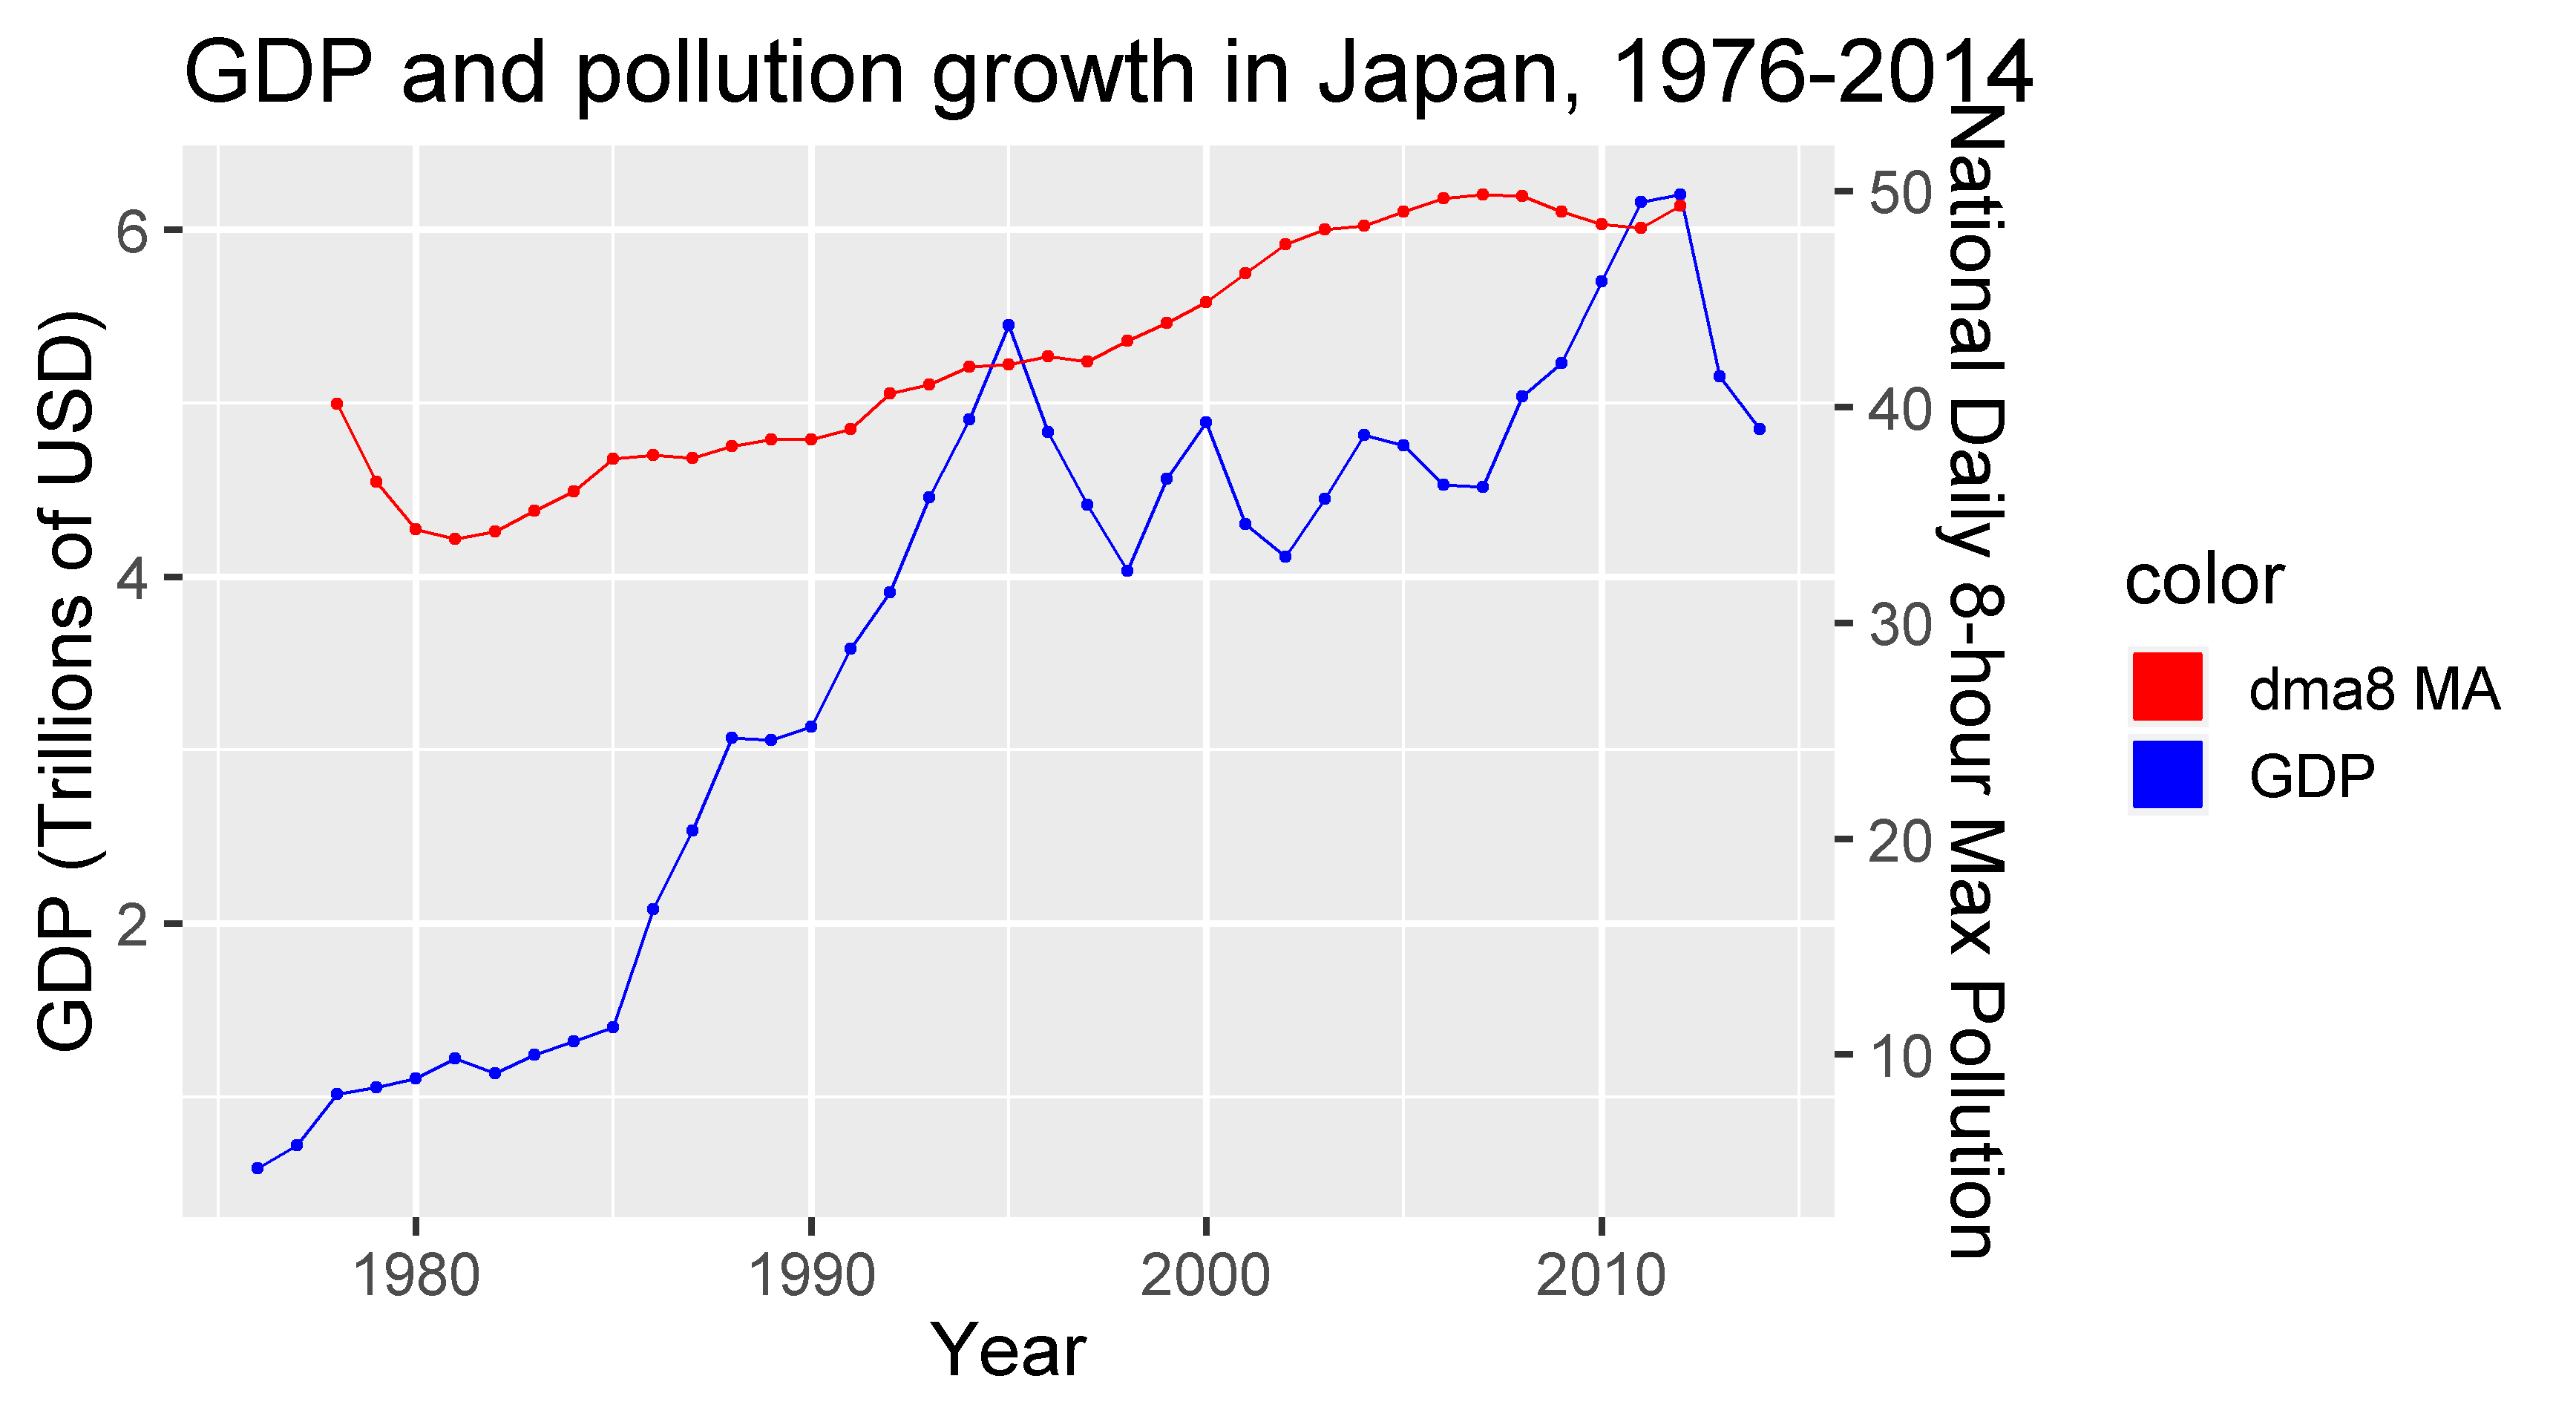
\includegraphics[width=0.45\linewidth]{plots/country_pollution/Japan_dma8.png}
    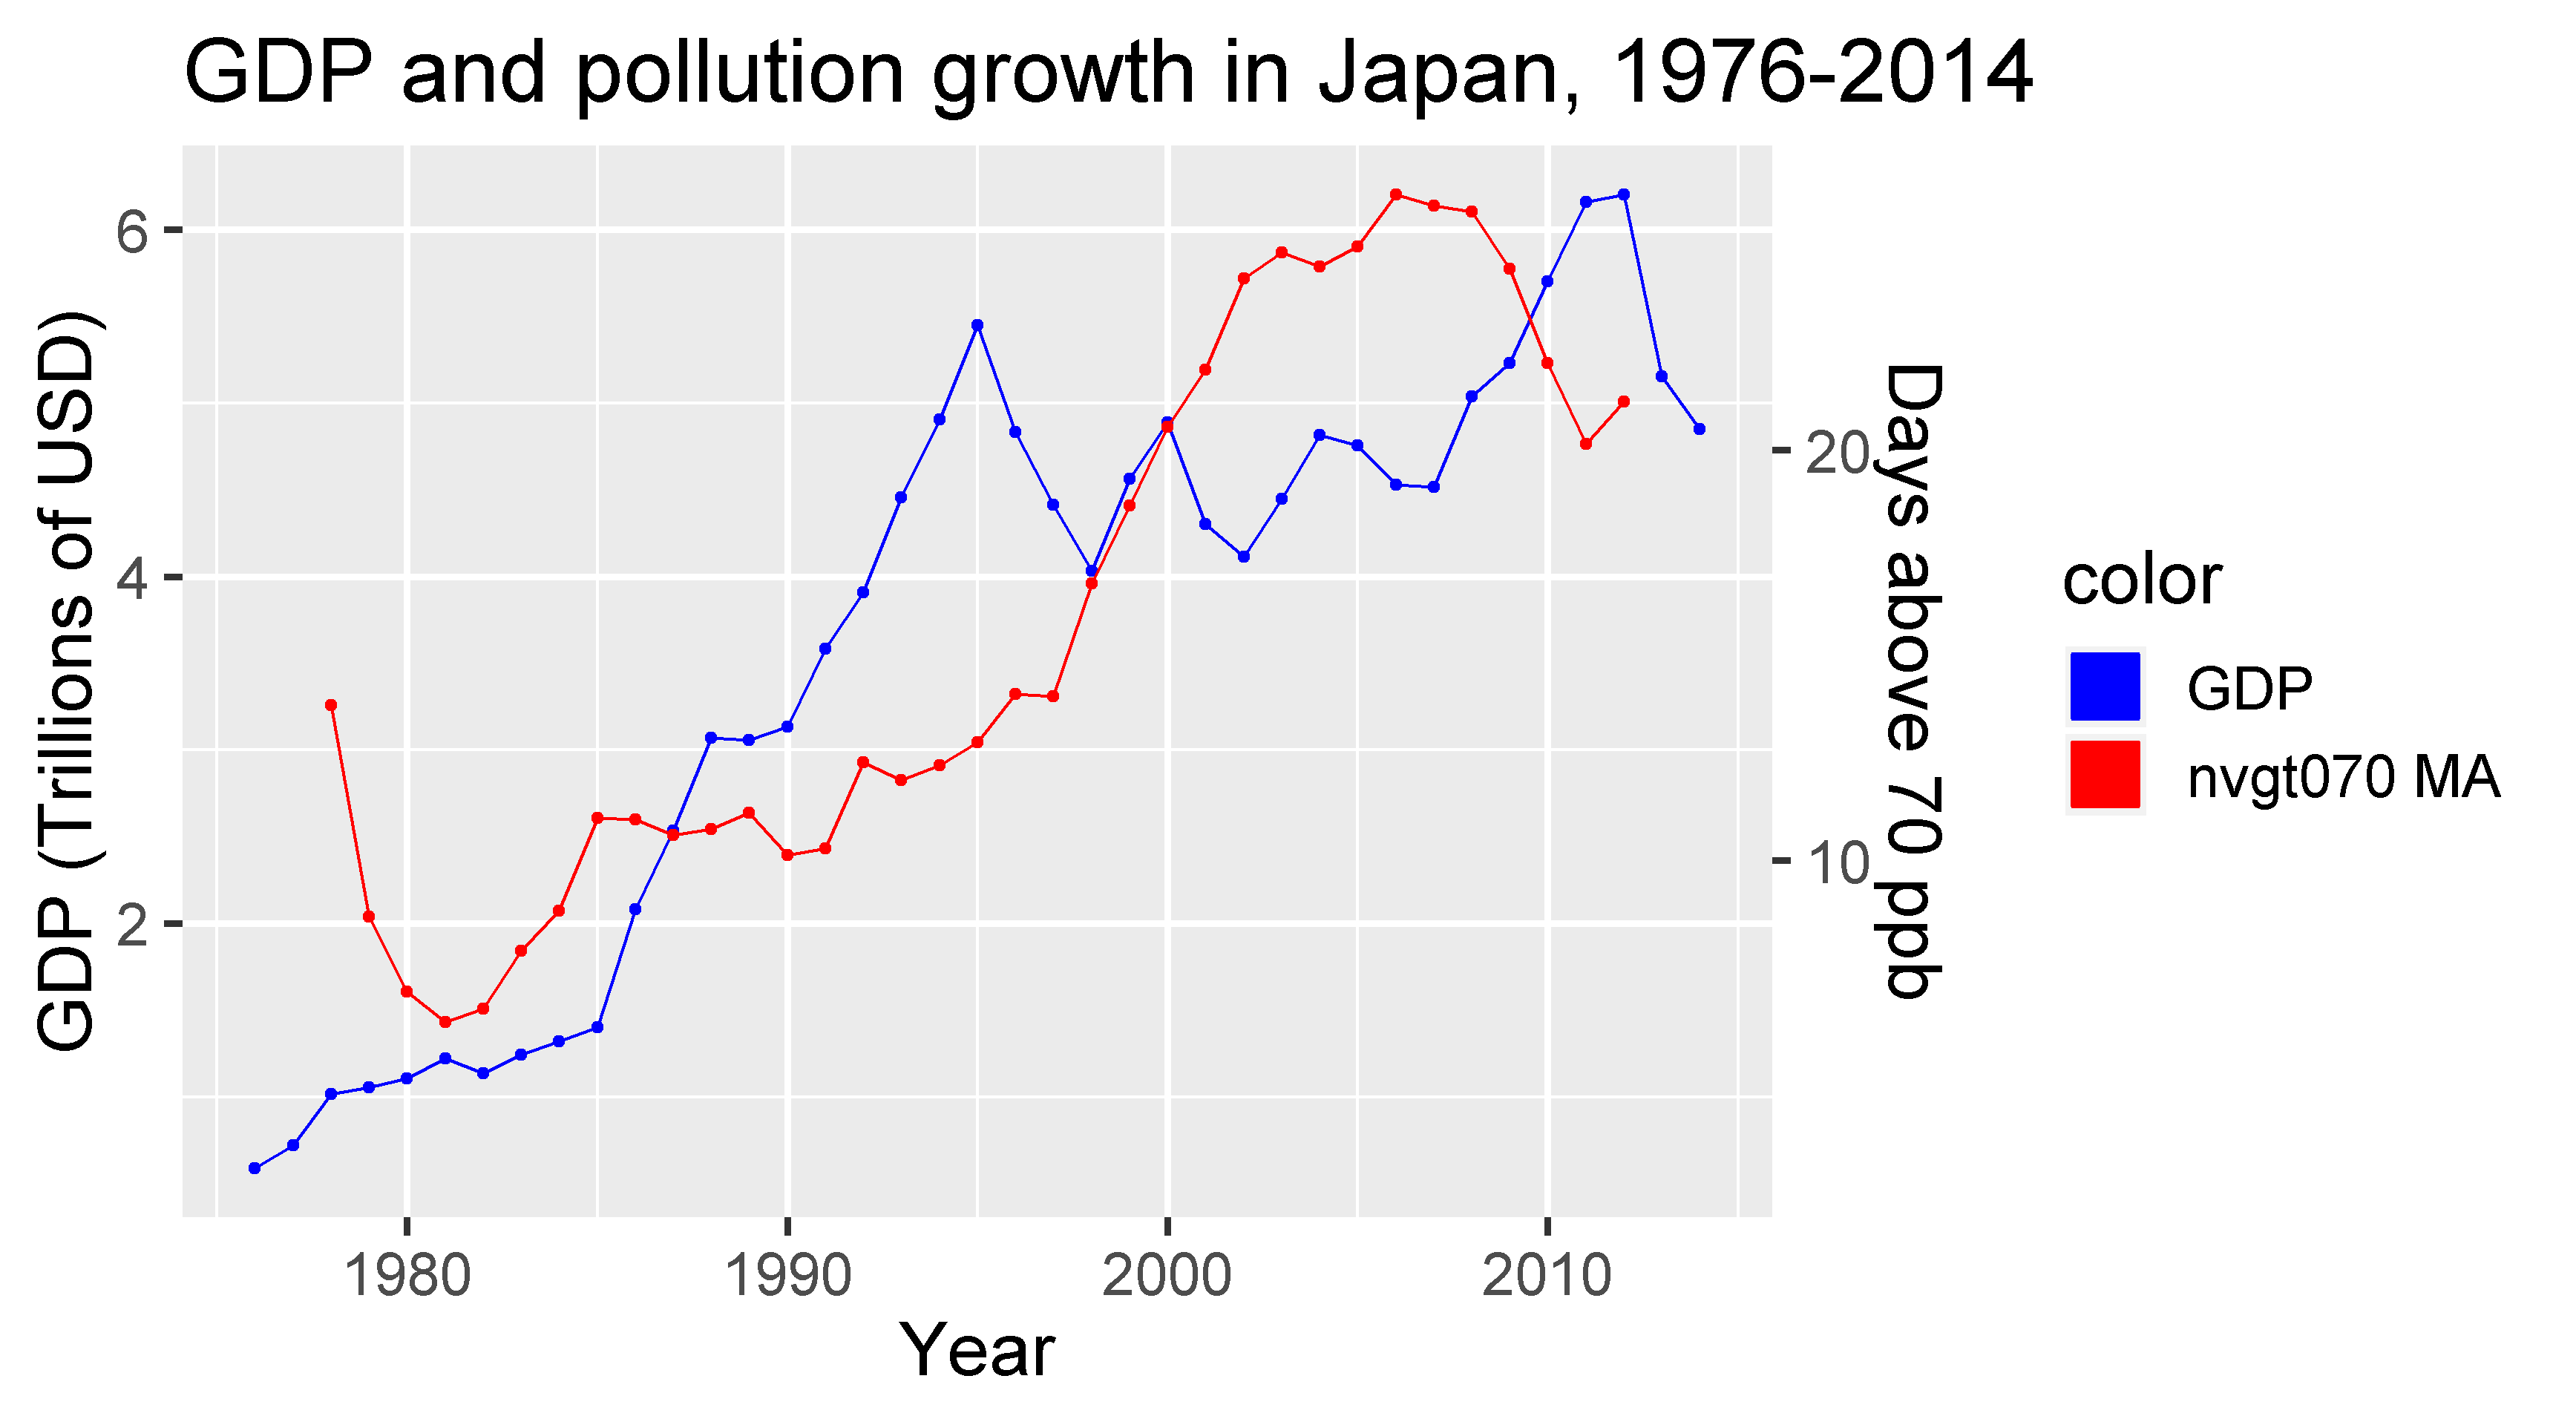
\includegraphics[width=0.45\linewidth]{plots/country_pollution/Japan_nvgt.png}
    %\caption{Japan}
    \label{fig:JP}
\end{figure}

In Japan we see a closer relationship between the ozone metrics and GDP. The mixing ratio, days above 70ppb, and GDP grew from 1970-1995, followed by a short period where the GDP plateaued and the metrics continued to rise. After about 2000, it appears that the ozone metrics also plateaued. 

\begin{figure}[ht]
    \centering
    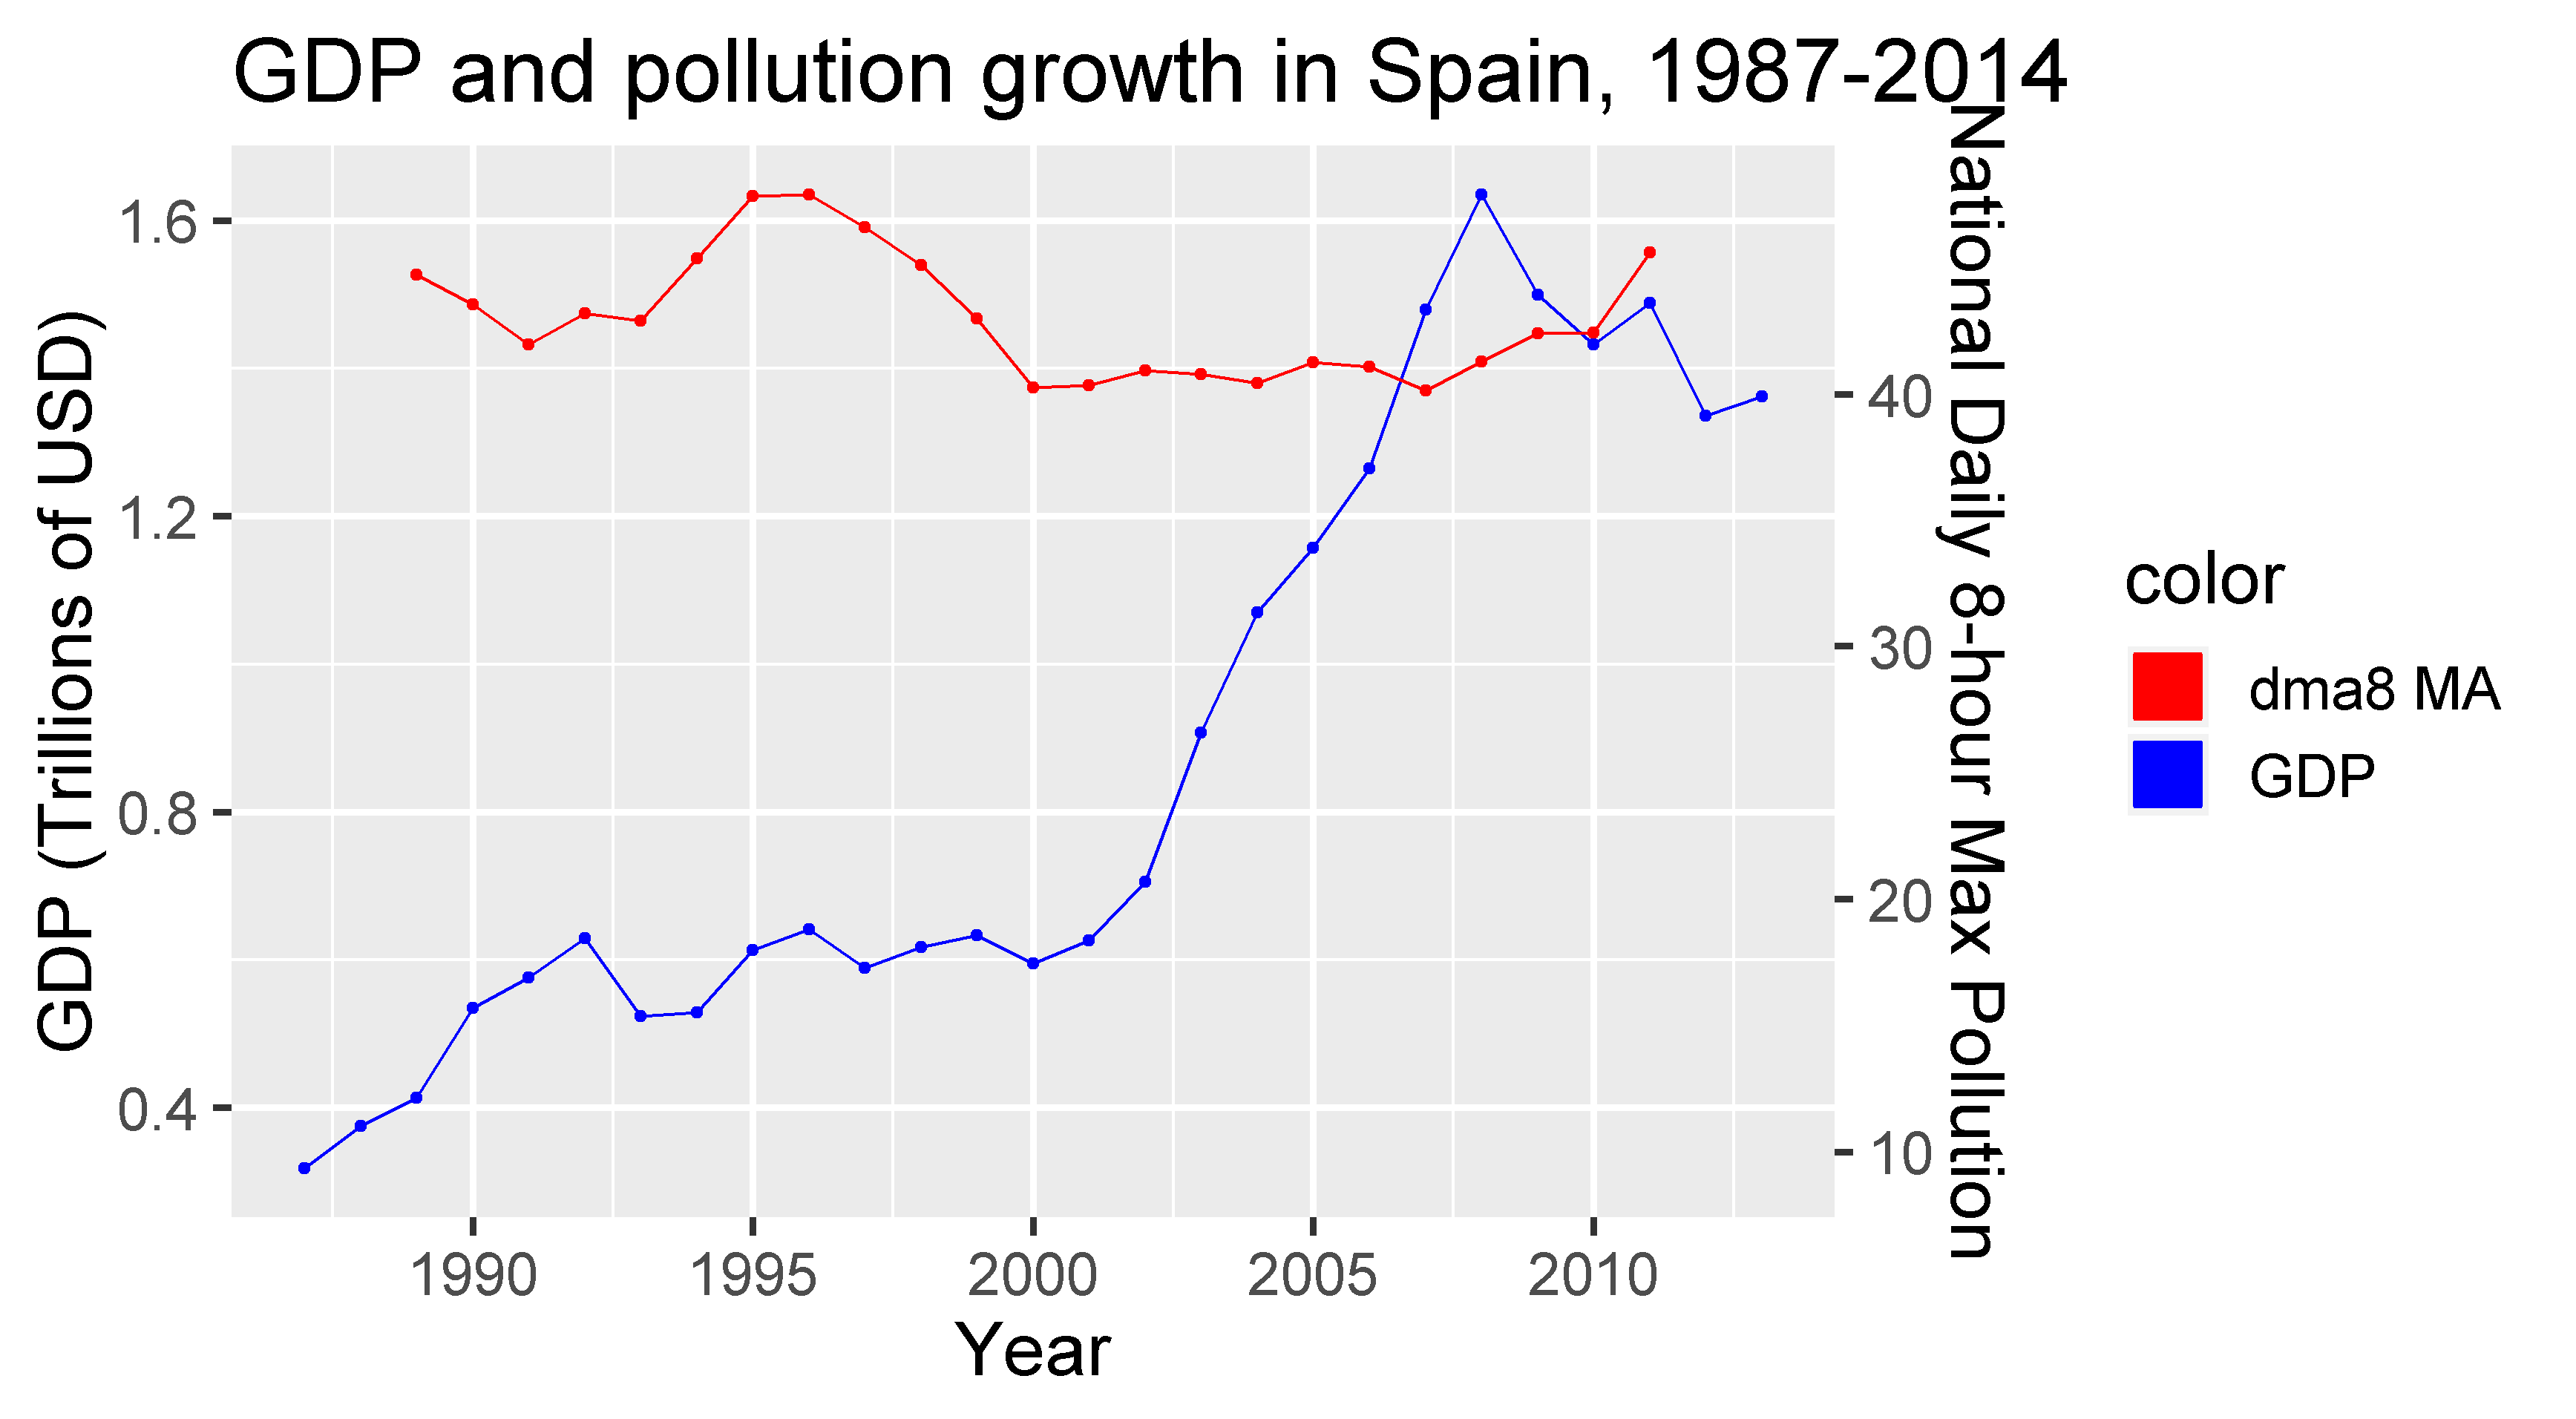
\includegraphics[width=0.45\linewidth]{plots/country_pollution/Spain_dma8.png}
    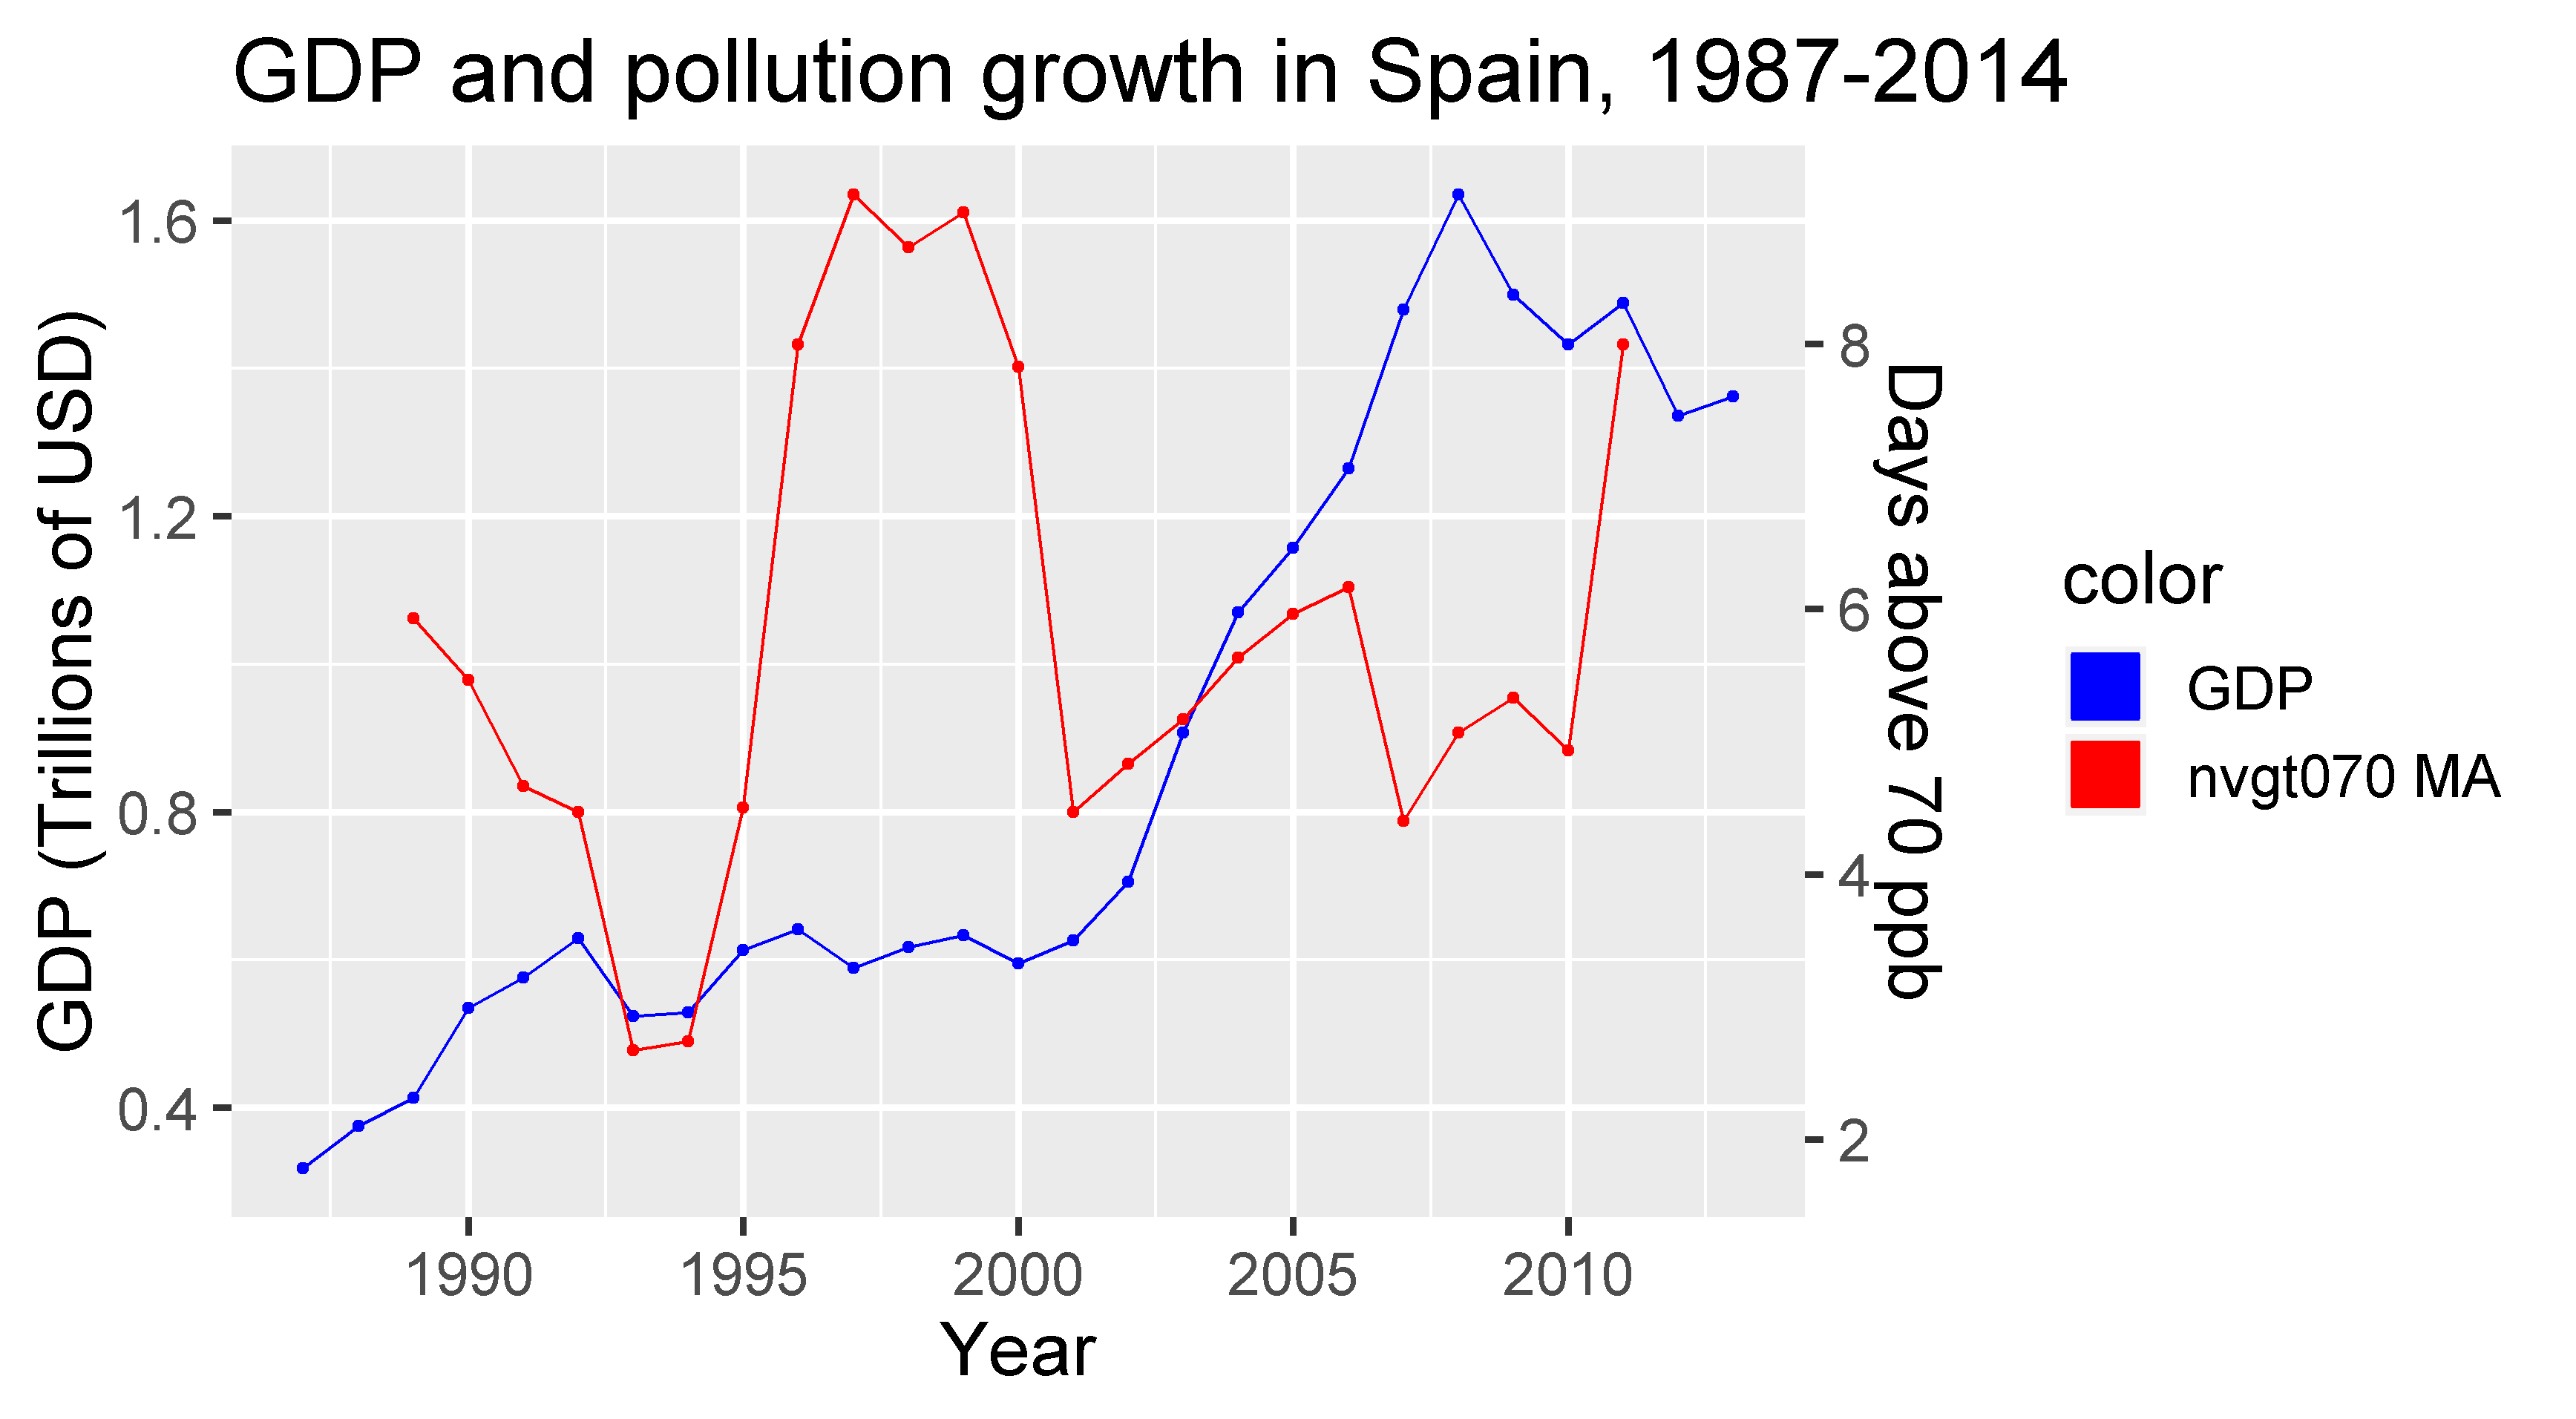
\includegraphics[width=0.45\linewidth]{plots/country_pollution/Spain_nvgt.png}
    %\caption{Spain}
    \label{fig:ESP}
\end{figure}

Spain's GDP has progressed differently from the other nations examined, having remained fairly steady before the year 2000 and growing rapidly for the better part of the decade after. The ozone metrics seem to not have much of a relationship with the GDP, as they had a peak in the 1990's and were at a relatively constant rate while the country's GDP skyrocketed.

%\begin{figure}[ht]
%    \centering
%    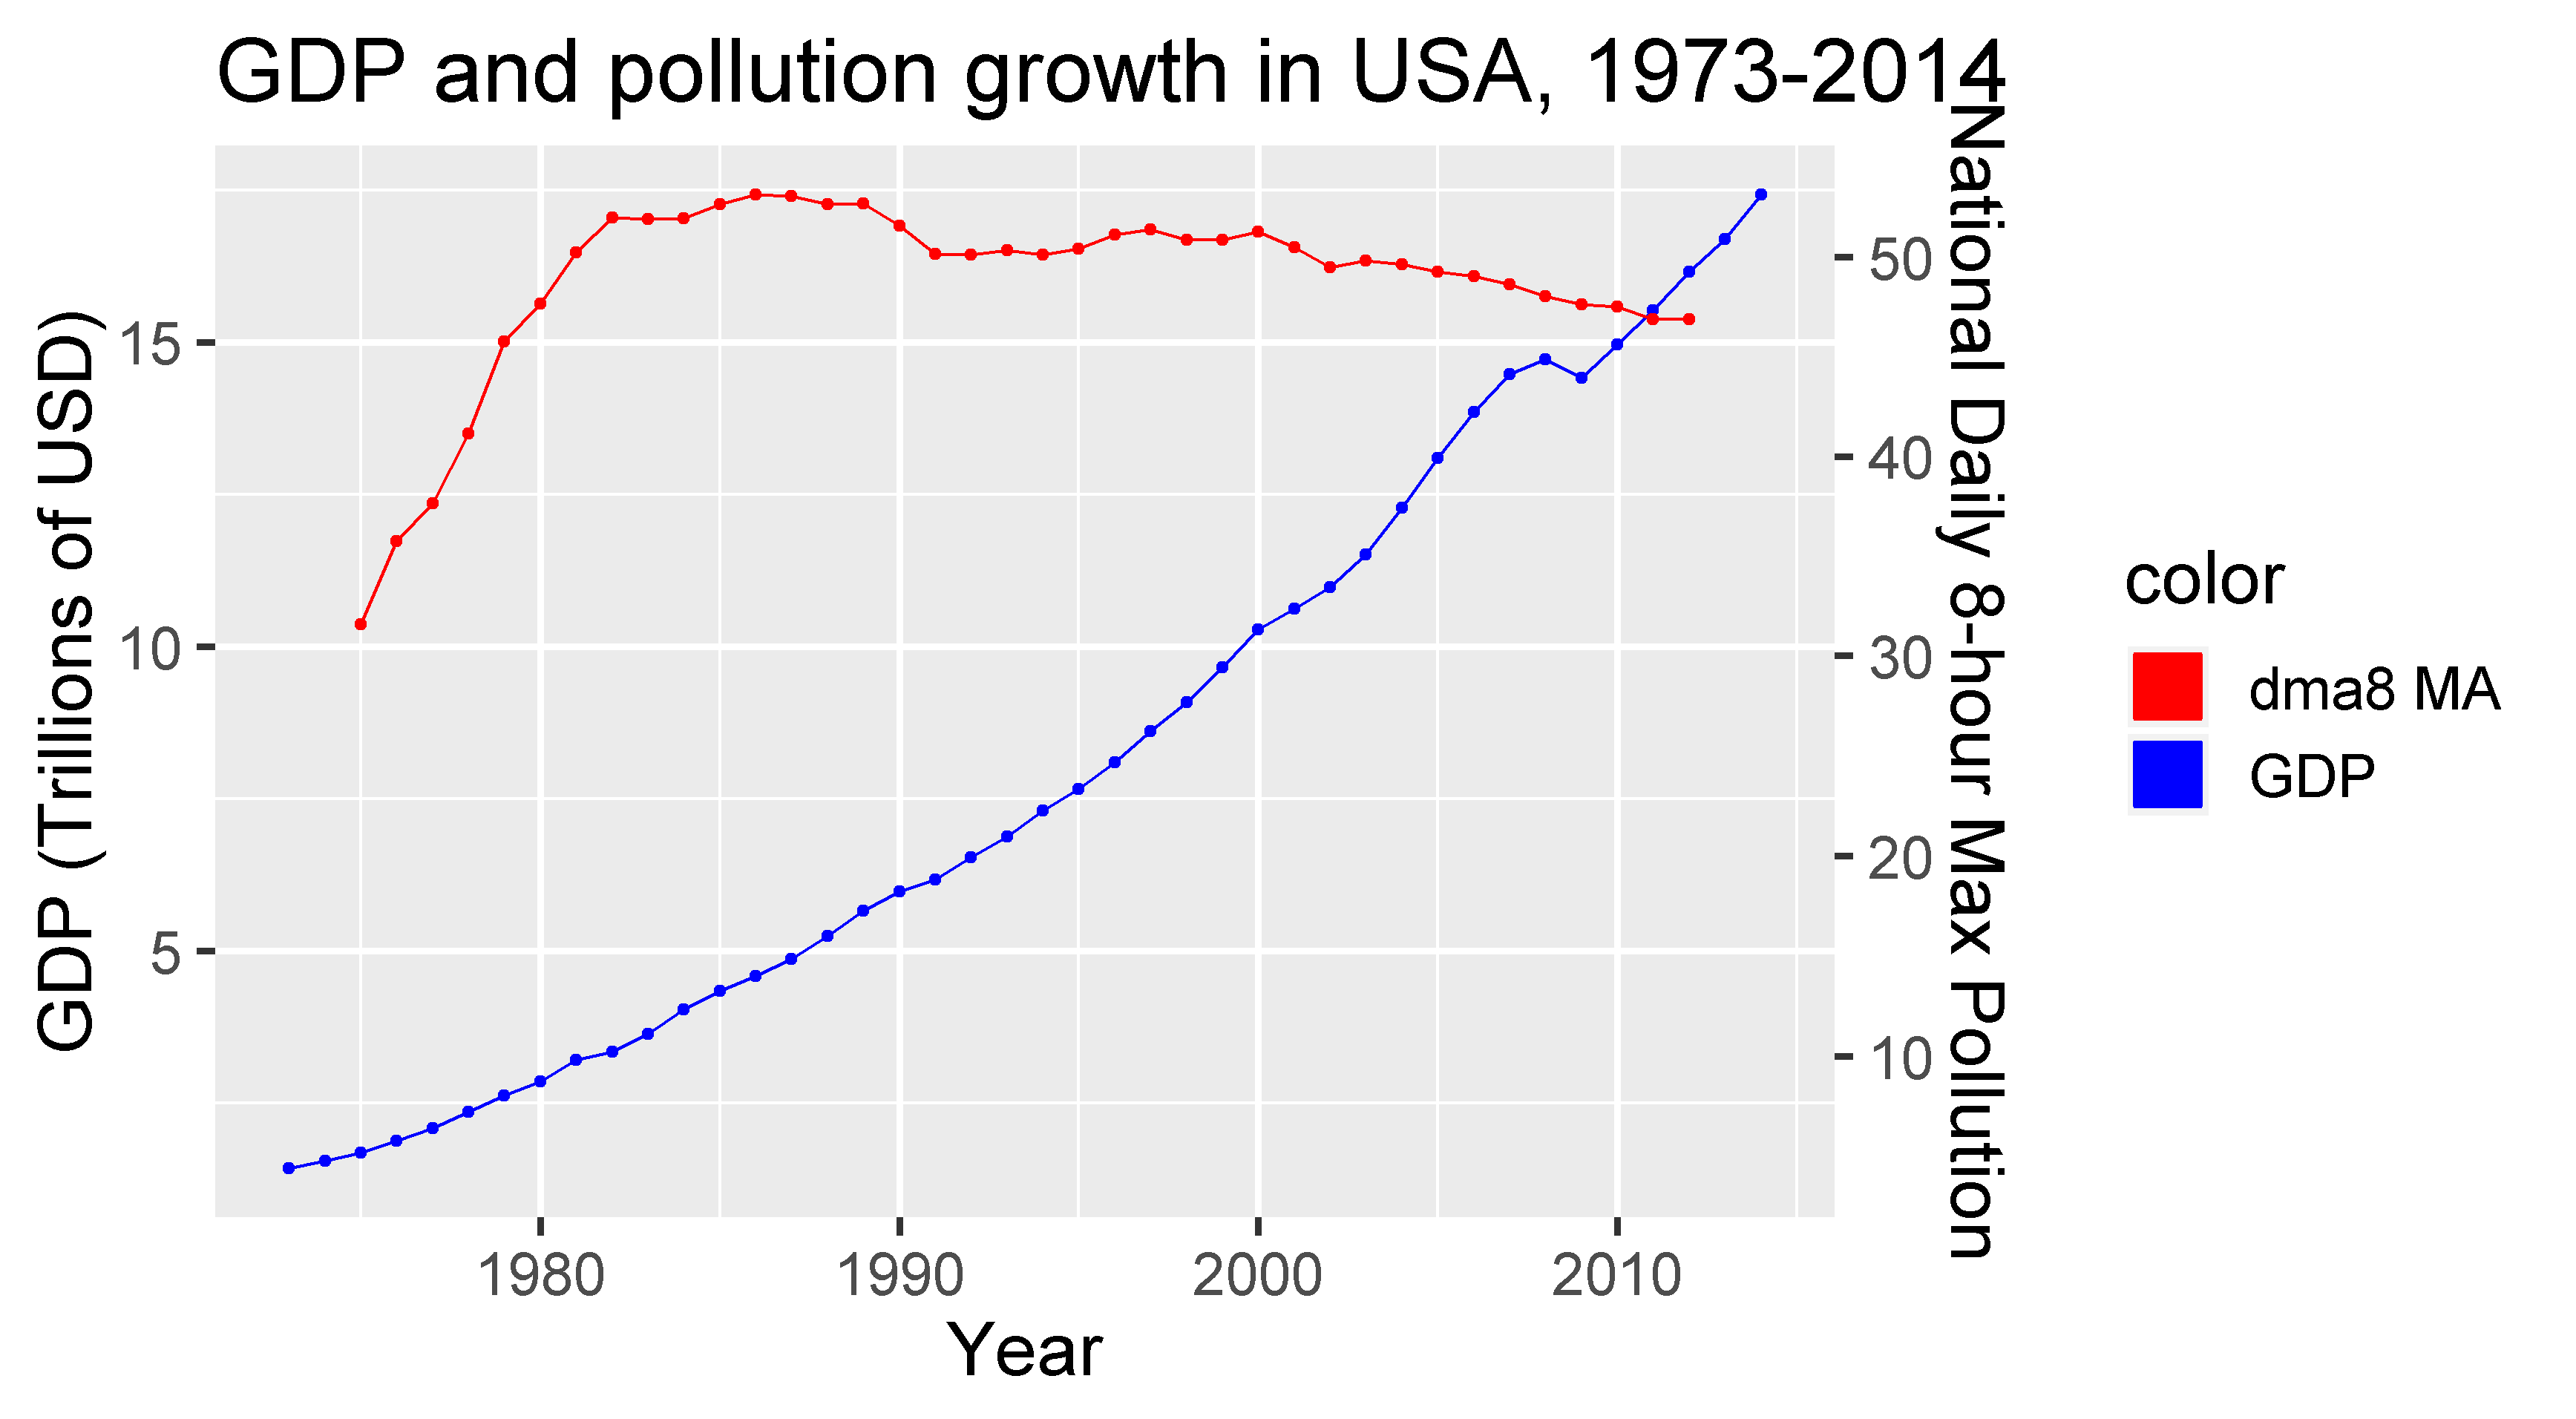
\includegraphics[width=0.45\linewidth]{plots/country_pollution/USA_dma8.png}
%    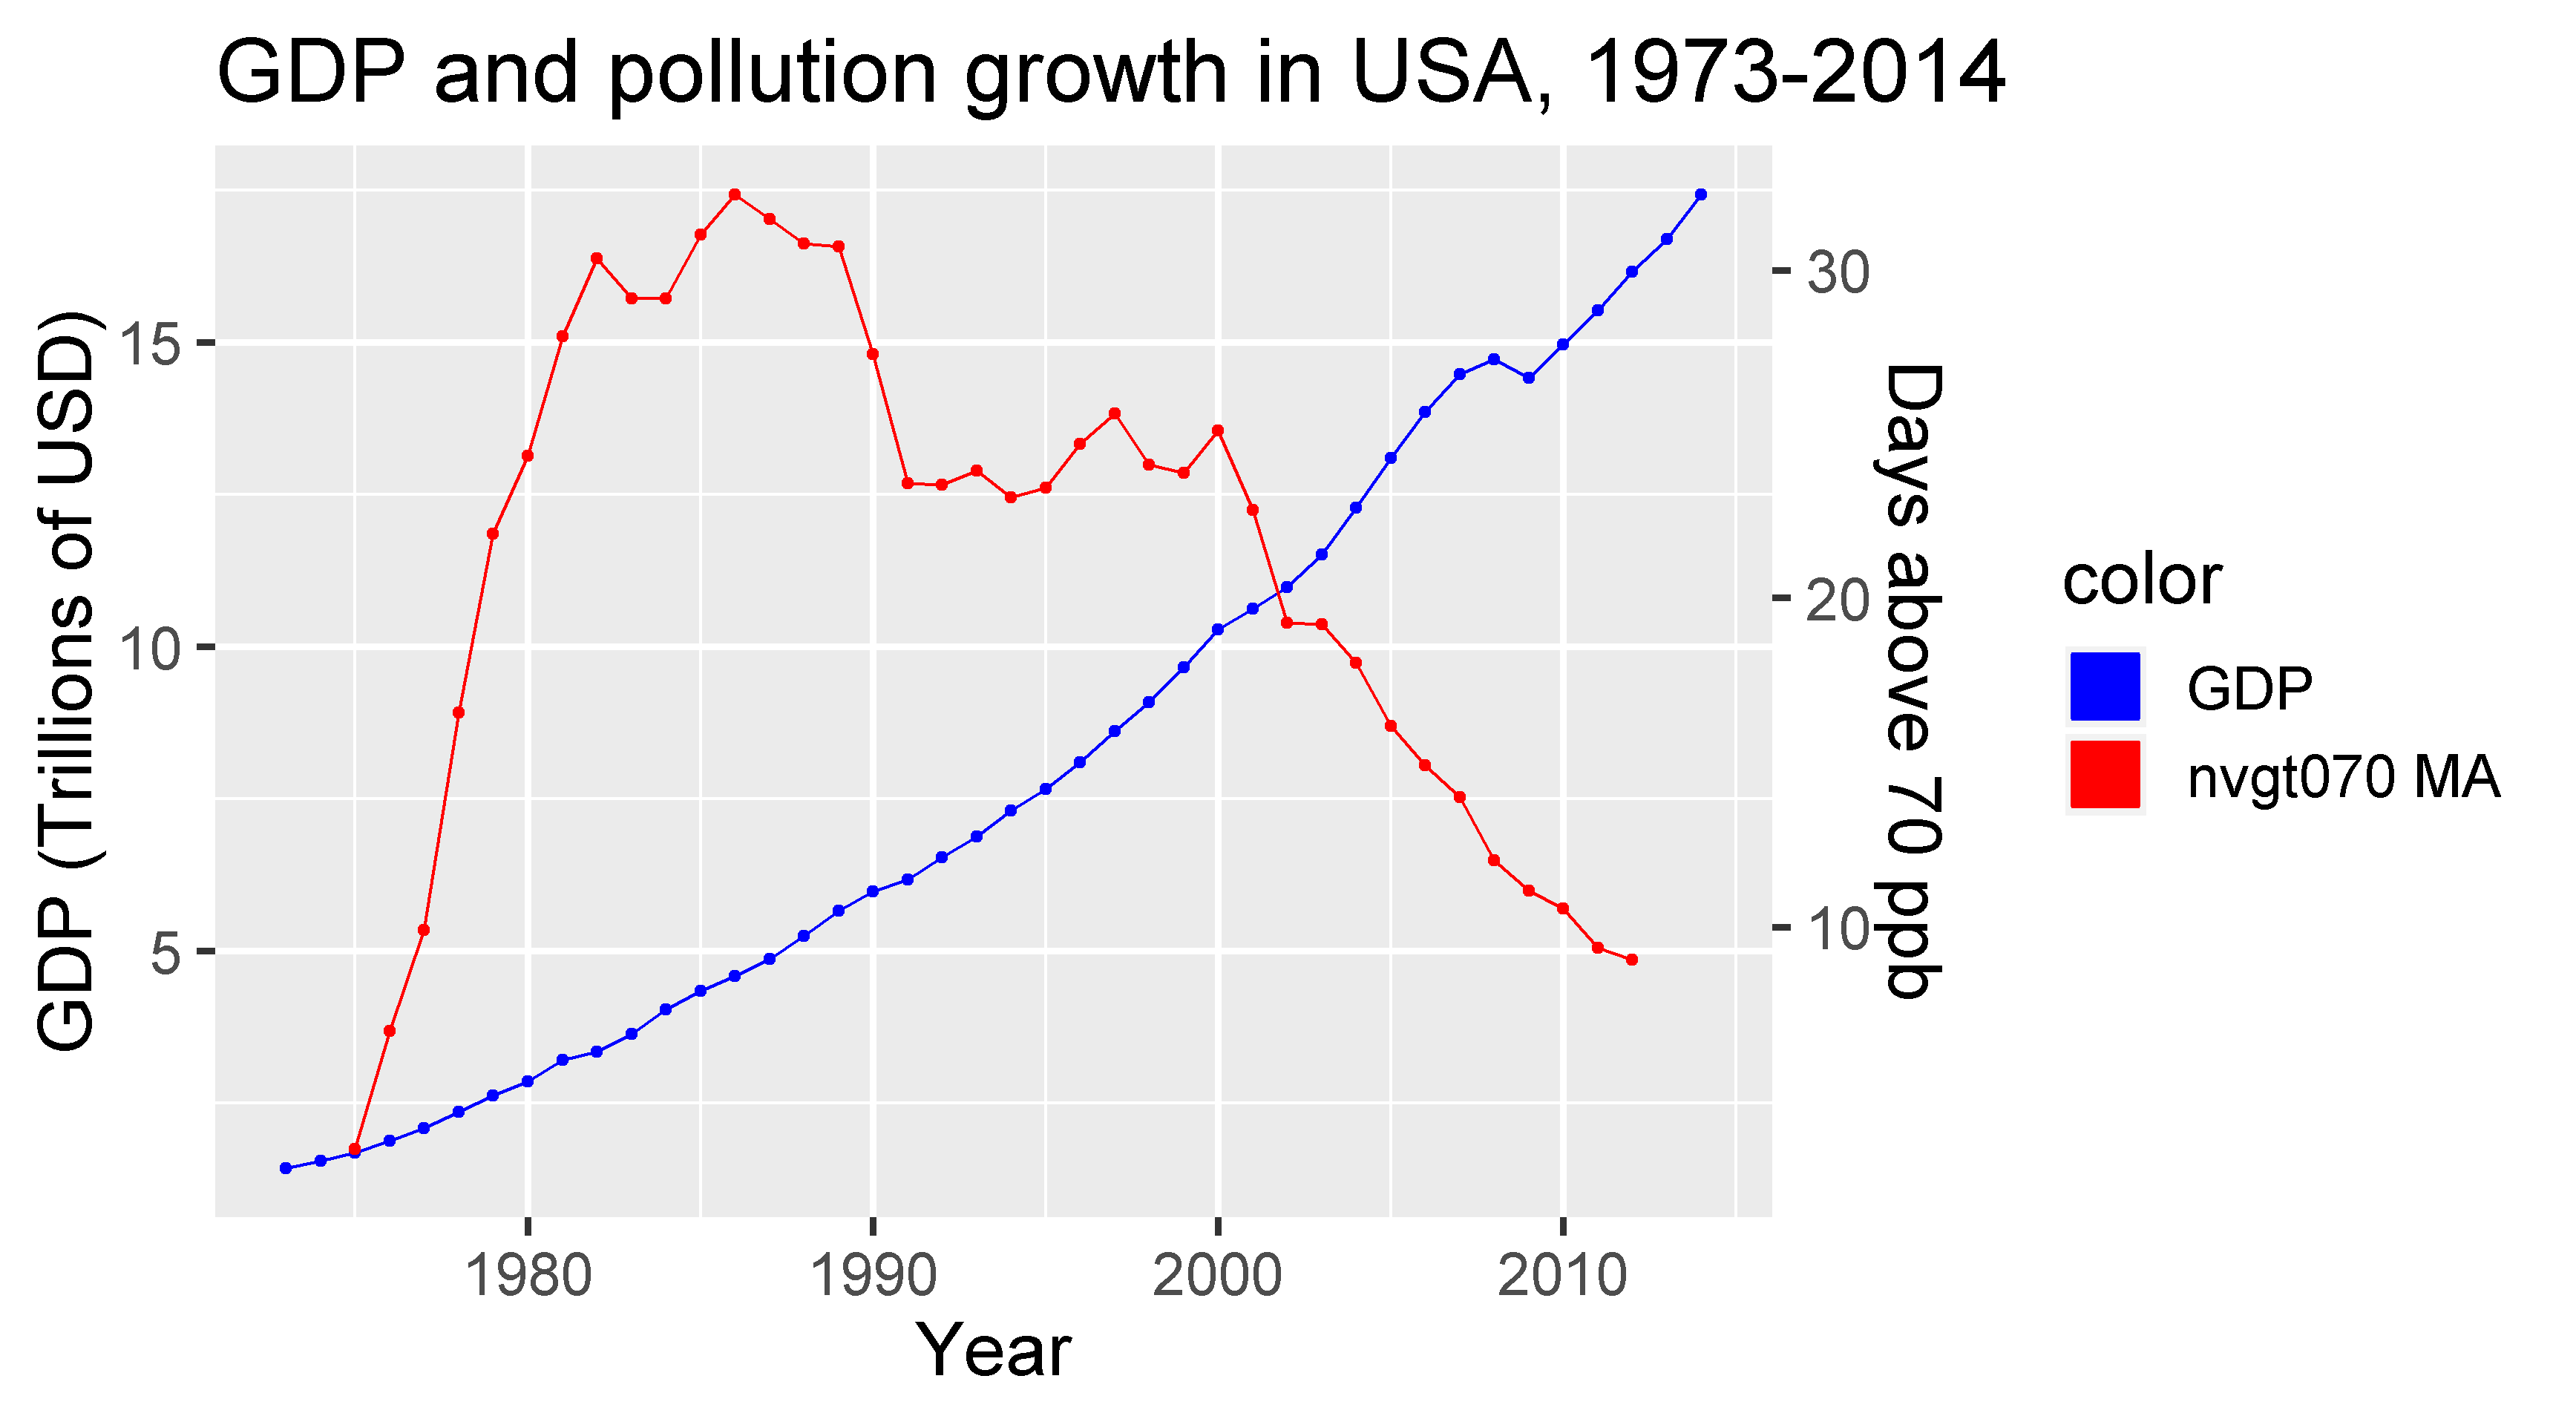
\includegraphics[width=0.45\linewidth]{plots/country_pollution/USA_nvgt.png}
    %\caption{US}
%    \label{fig:USA}
%\end{figure}

The United States has had the most consistent GDP growth of all of these nations, having grown in all years not affected by the 2008 recession. The pollution metrics both seem to grow until the early 1980's, after which they both began to decline. 

From analyzing these time series plots, it becomes more clear that a statistical model explaining worldwide ozone trends may not exist and that relationships may need to be explored on a more local level.  


%\section{Data}\label{sec:data}

%\section{Methods}\label{sec:methods}

%\section{Conclusion}

\newpage

\bibliographystyle{apalike}
\bibliography{techNote}


\end{document}